\documentclass[a4paper]{article}
\usepackage[utf8]{inputenc}
\usepackage{fullpage}

\usepackage[dvipsnames]{xcolor}
\usepackage{amsmath}
\usepackage{amssymb}
\usepackage{amsfonts}
\usepackage{amsthm}
\usepackage{graphicx}
\usepackage{tikz}
\usepackage{tikz-cd}
\usetikzlibrary{calc}
\usepackage{amscd}


\newtheorem{definition}{Definition}[section]
\newtheorem{theorem}{Theorem}[section]
\newtheorem{lemma}[theorem]{Lemma}
\newtheorem{remark}[theorem]{Remark}
\newtheorem{example}[theorem]{Example}
\newtheorem{proposition}[theorem]{Proposition}

\makeatletter
\newcommand\suchthat{%
 \@ifstar
  {\mathrel{}\middle|\mathrel{}}
  {\mid}%
}
\makeatother

\newcommand{\Ceins}[1]{C_{1,#1}}
\newcommand{\Czwei}[1]{C_{2,#1}}
\newcommand{\Cdrei}[1]{C_{3,#1}}
\newcommand{\Cvier}[2]{C_{4,#1,#2}}
\newcommand{\Cfive}[2]{C_{5,#1,#2}}
% \newcommand{\Ceins}{\sqrt{n}}
% \newcommand{\Czwei}{\sqrt{2n}}



\newcommand{\Perm}{{\operatorname{Perm}}}

\newcommand{\linhull}{{\operatorname{span}}}
\newcommand{\convexhull}{{\operatorname{convex}}}

\newcommand{\Poinc}{\frakP}
\newcommand{\Bogov}{\frakB}

\newcommand{\mollifier}{\frakm}

\newcommand{\eps}{\epsilon}

\newcommand{\Id}{\rm{Id}}

\newcommand{\Lip}{\rm{Lip}}

\newcommand{\diff}{\mathop{}\!\mathrm{d}}

\DeclareMathOperator{\adj}{adj}
%\newcommand{\adj}{{\rm adj}}
\newcommand{\inv}{{-1}}
\newcommand{\invt}{{-t}}
\newcommand{\tinv}{{-t}}
\newcommand{\determinant}{{\operatorname{det}}}
\DeclareMathOperator{\Jacobian}{{\rm Jac}}
% \newcommand{\Jacobian}{{\rm Jac}}
\newcommand{\dimension}{\operatorname{dim}}
\newcommand{\sgn}{\operatorname{sgn}}
\newcommand{\adjugate}{\operatorname{adj}}
\newcommand{\sym}{\operatorname{sym}}
\newcommand{\signum}{\operatorname{sgn}}
\newcommand{\kronecker}{{\hat\delta}}
\newcommand{\dom}{\operatorname{dom}}
\newcommand{\codom}{\operatorname{codom}}
\newcommand{\rng}{\operatorname{ran}}
\newcommand{\convex}{\operatorname{convex}}
\newcommand{\coker}{\operatorname{coker}}
\newcommand{\coran}{\operatorname{coran}}

\newcommand{\dif}{{\mathrm d}}
\newcommand{\Dif}{{\mathrm D}}
\newcommand{\grad}{\operatorname{grad}}
\newcommand{\Grad}{\operatorname{Grad}}
\newcommand{\curl}{\operatorname{curl}}
\newcommand{\Curl}{\operatorname{Curl}}
\newcommand{\rot}{\curl}
\newcommand{\divergence}{\operatorname{div}}
\newcommand{\diver}{\operatorname{div}}
\newcommand{\svcurl}{\operatorname{sv-curl}}
\newcommand{\vscurl}{\operatorname{vs-curl}}
\newcommand{\sdiver}{\operatorname{sdiv}}
\newcommand{\Sdiver}{\operatorname{Sdiv}}
\newcommand{\sgrad}{\operatorname{sgrad}}
\newcommand{\Sgrad}{\operatorname{Sgrad}}
\newcommand{\Laplace}{\bigtriangleup}
\newcommand{\laplace}{\bigtriangleup}
\newcommand{\laplacian}{\laplace}
\newcommand{\Laplacian}{\laplace}
% \newcommand{\cartan}{{\mathsf d}}
% \newcommand{\cartanx}{{\mathsf d}x}
\newcommand{\cartan}{d}
\newcommand{\cartanx}{dx}

%\newcommand{\argmin}{\operatorname{argmin}}
\DeclareMathOperator*{\argmin}{{\rm argmin}}

% \DeclareMathOperator*{\carapace}{{\rm corona}}
\DeclareMathOperator*{\carapace}{{\partial \rm st}}

\newcommand{\supp}{\operatorname{supp}}
\newcommand{\esssup}{{\operatorname{esssup}}}
\newcommand{\essinf}{{\operatorname{essinf}}}

\newcommand{\equivalent}{ \Longleftrightarrow }
\newcommand{\vol}{\operatorname{vol}}
\newcommand{\st}{ \mid }
\newcommand{\diam}{{\operatorname{diam}}}
\newcommand{\height}{\operatorname{height}}
\newcommand{\dist}{\operatorname{dist}}
\newcommand{\patch}{\operatorname{st}}

\newcommand{\Trace}{\operatorname{Tr}}
\newcommand{\Tr}{\operatorname{Tr}}
\newcommand{\trace}{\operatorname{tr}}
\newcommand{\normaltrace}{\operatorname{nm}}
\newcommand{\tr}{\operatorname{tr}}
\newcommand{\Ext}{\operatorname{Ext}}
\newcommand{\Ex}{\operatorname{Ex}}
\newcommand{\ext}{\operatorname{ext}}

\newcommand{\Poincare}{\sfP}
\newcommand*{\volsphere}[1]{\color{red}{S_{#1}}}
\newcommand*{\volball}[1]{B_{#1}}

\newcommand{\subsimplex}{\calS^{\downarrow}}
\newcommand{\supsimplex}{\calS^{\uparrow}}
\newcommand{\supersimplex}{\supsimplex}
\newcommand{\orientation}{\mathscr{O}}
\newcommand{\restrict}{R}

\newcommand{\Mesh}{\calT}
\newcommand{\Vertices}{\calV}
\newcommand{\Edges}{\calE}
\newcommand{\Faces}{\calF}
\newcommand{\Ball}{\calB}
\newcommand{\Sphere}{S}
\newcommand{\underlying}[1]{\left| #1 \right|}

\newcommand{\Distr}{\calD}
\newcommand{\Cont}{\calC}
\newcommand{\Lebesgue}{L}
\newcommand{\Sobolev}{W}
\newcommand{\SOBOLEV}{\bfW}
\newcommand{\SobolevLambda}{W\Lambda}
\newcommand{\Alt}{\Lambda}
\newcommand{\loc}{\rm{loc}}

\newcommand{\Ned}{{\calN d}}
\newcommand{\RT}{{\calR T}}
\newcommand{\BDM}{{\calB \calD \calM}}
  

\newcommand*{\ConstantPF}{C_{\rm{PF}}}







\newcommand{\bbA}{{\mathbb A}}
\newcommand{\bbB}{{\mathbb B}}
\newcommand{\bbC}{{\mathbb C}}
\newcommand{\bbD}{{\mathbb D}}
\newcommand{\bbE}{{\mathbb E}}
\newcommand{\bbF}{{\mathbb F}}
\newcommand{\bbG}{{\mathbb G}}
\newcommand{\bbH}{{\mathbb H}}
\newcommand{\bbI}{{\mathbb I}}
\newcommand{\bbJ}{{\mathbb J}}
\newcommand{\bbK}{{\mathbb K}}
\newcommand{\bbL}{{\mathbb L}}
\newcommand{\bbM}{{\mathbb M}}
\newcommand{\bbN}{{\mathbb N}}
\newcommand{\bbO}{{\mathbb O}}
\newcommand{\bbP}{{\mathbb P}}
\newcommand{\bbQ}{{\mathbb Q}}
\newcommand{\bbR}{{\mathbb R}}
\newcommand{\bbS}{{\mathbb S}}
\newcommand{\bbT}{{\mathbb T}}
\newcommand{\bbU}{{\mathbb U}}
\newcommand{\bbV}{{\mathbb V}}
\newcommand{\bbW}{{\mathbb W}}
\newcommand{\bbX}{{\mathbb X}}
\newcommand{\bbY}{{\mathbb Y}}
\newcommand{\bbZ}{{\mathbb Z}}

\newcommand{\bfA}{{\mathbf A}}
\newcommand{\bfB}{{\mathbf B}}
\newcommand{\bfC}{{\mathbf C}}
\newcommand{\bfD}{{\mathbf D}}
\newcommand{\bfE}{{\mathbf E}}
\newcommand{\bfF}{{\mathbf F}}
\newcommand{\bfG}{{\mathbf G}}
\newcommand{\bfH}{{\mathbf H}}
\newcommand{\bfI}{{\mathbf I}}
\newcommand{\bfJ}{{\mathbf J}}
\newcommand{\bfK}{{\mathbf K}}
\newcommand{\bfL}{{\mathbf L}}
\newcommand{\bfM}{{\mathbf M}}
\newcommand{\bfN}{{\mathbf N}}
\newcommand{\bfO}{{\mathbf O}}
\newcommand{\bfP}{{\mathbf P}}
\newcommand{\bfQ}{{\mathbf Q}}
\newcommand{\bfR}{{\mathbf R}}
\newcommand{\bfS}{{\mathbf S}}
\newcommand{\bfT}{{\mathbf T}}
\newcommand{\bfU}{{\mathbf U}}
\newcommand{\bfV}{{\mathbf V}}
\newcommand{\bfW}{{\mathbf W}}
\newcommand{\bfX}{{\mathbf X}}
\newcommand{\bfY}{{\mathbf Y}}
\newcommand{\bfZ}{{\mathbf Z}}

\newcommand{\bfa}{{\mathbf a}}
\newcommand{\bfb}{{\mathbf b}}
\newcommand{\bfc}{{\mathbf c}}
\newcommand{\bfd}{{\mathbf d}}
\newcommand{\bfe}{{\mathbf e}}
\newcommand{\bff}{{\mathbf f}}
\newcommand{\bfg}{{\mathbf g}}
\newcommand{\bfh}{{\mathbf h}}
\newcommand{\bfi}{{\mathbf i}}
\newcommand{\bfj}{{\mathbf j}}
\newcommand{\bfk}{{\mathbf k}}
\newcommand{\bfl}{{\mathbf l}}
\newcommand{\bfm}{{\mathbf m}}
\newcommand{\bfn}{{\mathbf n}}
\newcommand{\bfo}{{\mathbf o}}
\newcommand{\bfp}{{\mathbf p}}
\newcommand{\bfq}{{\mathbf q}}
\newcommand{\bfr}{{\mathbf r}}
\newcommand{\bfs}{{\mathbf s}}
\newcommand{\bft}{{\mathbf t}}
\newcommand{\bfu}{{\mathbf u}}
\newcommand{\bfv}{{\mathbf v}}
\newcommand{\bfw}{{\mathbf w}}
\newcommand{\bfx}{{\mathbf x}}
\newcommand{\bfy}{{\mathbf y}}
\newcommand{\bfz}{{\mathbf z}}


\newcommand{\calA}{{\mathcal A}}
\newcommand{\calB}{{\mathcal B}}
\newcommand{\calC}{{\mathcal C}}
\newcommand{\calD}{{\mathcal D}}
\newcommand{\calE}{{\mathcal E}}
\newcommand{\calF}{{\mathcal F}}
\newcommand{\calG}{{\mathcal G}}
\newcommand{\calH}{{\mathcal H}}
\newcommand{\calI}{{\mathcal I}}
\newcommand{\calJ}{{\mathcal J}}
\newcommand{\calK}{{\mathcal K}}
\newcommand{\calL}{{\mathcal L}}
\newcommand{\calM}{{\mathcal M}}
\newcommand{\calN}{{\mathcal N}}
\newcommand{\calO}{{\mathcal O}}
\newcommand{\calP}{{\mathcal P}}
\newcommand{\calQ}{{\mathcal Q}}
\newcommand{\calR}{{\mathcal R}}
\newcommand{\calS}{{\mathcal S}}
\newcommand{\calT}{{\mathcal T}}
\newcommand{\calU}{{\mathcal U}}
\newcommand{\calV}{{\mathcal V}}
\newcommand{\calW}{{\mathcal W}}
\newcommand{\calX}{{\mathcal X}}
\newcommand{\calY}{{\mathcal Y}}
\newcommand{\calZ}{{\mathcal Z}}

\newcommand{\fraka}{{\mathfrak a}}
\newcommand{\frakb}{{\mathfrak b}}
\newcommand{\frakc}{{\mathfrak c}}
\newcommand{\frakd}{{\mathfrak d}}
\newcommand{\frake}{{\mathfrak e}}
\newcommand{\frakf}{{\mathfrak f}}
\newcommand{\frakg}{{\mathfrak g}}
\newcommand{\frakh}{{\mathfrak h}}
\newcommand{\fraki}{{\mathfrak i}}
\newcommand{\frakj}{{\mathfrak j}}
\newcommand{\frakk}{{\mathfrak k}}
\newcommand{\frakl}{{\mathfrak l}}
\newcommand{\frakm}{{\mathfrak m}}
\newcommand{\frakn}{{\mathfrak n}}
\newcommand{\frako}{{\mathfrak o}}
\newcommand{\frakp}{{\mathfrak p}}
\newcommand{\frakq}{{\mathfrak q}}
\newcommand{\frakr}{{\mathfrak r}}
\newcommand{\fraks}{{\mathfrak s}}
\newcommand{\frakt}{{\mathfrak t}}
\newcommand{\fraku}{{\mathfrak u}}
\newcommand{\frakv}{{\mathfrak v}}
\newcommand{\frakw}{{\mathfrak w}}
\newcommand{\frakx}{{\mathfrak x}}
\newcommand{\fraky}{{\mathfrak y}}
\newcommand{\frakz}{{\mathfrak z}}
\newcommand{\frakA}{{\mathfrak A}}
\newcommand{\frakB}{{\mathfrak B}}
\newcommand{\frakC}{{\mathfrak C}}
\newcommand{\frakD}{{\mathfrak D}}
\newcommand{\frakE}{{\mathfrak E}}
\newcommand{\frakF}{{\mathfrak F}}
\newcommand{\frakG}{{\mathfrak G}}
\newcommand{\frakH}{{\mathfrak H}}
\newcommand{\frakI}{{\mathfrak I}}
\newcommand{\frakJ}{{\mathfrak J}}
\newcommand{\frakK}{{\mathfrak K}}
\newcommand{\frakL}{{\mathfrak L}}
\newcommand{\frakM}{{\mathfrak M}}
\newcommand{\frakN}{{\mathfrak N}}
\newcommand{\frakO}{{\mathfrak O}}
\newcommand{\frakP}{{\mathfrak P}}
\newcommand{\frakQ}{{\mathfrak Q}}
\newcommand{\frakR}{{\mathfrak R}}
\newcommand{\frakS}{{\mathfrak S}}
\newcommand{\frakT}{{\mathfrak T}}
\newcommand{\frakU}{{\mathfrak U}}
\newcommand{\frakV}{{\mathfrak V}}
\newcommand{\frakW}{{\mathfrak W}}
\newcommand{\frakX}{{\mathfrak X}}
\newcommand{\frakY}{{\mathfrak Y}}
\newcommand{\frakZ}{{\mathfrak Z}}







\newcommand{\rma}{{\mathrm a}}
\newcommand{\rmb}{{\mathrm b}}
\newcommand{\rmc}{{\mathrm c}}
\newcommand{\rmd}{{\mathrm d}}
\newcommand{\rme}{{\mathrm e}}
\newcommand{\rmf}{{\mathrm f}}
\newcommand{\rmg}{{\mathrm g}}
\newcommand{\rmh}{{\mathrm h}}
\newcommand{\rmi}{{\mathrm i}}
\newcommand{\rmj}{{\mathrm j}}
\newcommand{\rmk}{{\mathrm k}}
\newcommand{\rml}{{\mathrm l}}
\newcommand{\rmm}{{\mathrm m}}
\newcommand{\rmn}{{\mathrm n}}
\newcommand{\rmo}{{\mathrm o}}
\newcommand{\rmp}{{\mathrm p}}
\newcommand{\rmq}{{\mathrm q}}
\newcommand{\rmr}{{\mathrm r}}
\newcommand{\rms}{{\mathrm s}}
\newcommand{\rmt}{{\mathrm t}}
\newcommand{\rmu}{{\mathrm u}}
\newcommand{\rmv}{{\mathrm v}}
\newcommand{\rmw}{{\mathrm w}}
\newcommand{\rmx}{{\mathrm x}}
\newcommand{\rmy}{{\mathrm y}}
\newcommand{\rmz}{{\mathrm z}}
\newcommand{\rmA}{{\mathrm A}}
\newcommand{\rmB}{{\mathrm B}}
\newcommand{\rmC}{{\mathrm C}}
\newcommand{\rmD}{{\mathrm D}}
\newcommand{\rmE}{{\mathrm E}}
\newcommand{\rmF}{{\mathrm F}}
\newcommand{\rmG}{{\mathrm G}}
\newcommand{\rmH}{{\mathrm H}}
\newcommand{\rmI}{{\mathrm I}}
\newcommand{\rmJ}{{\mathrm J}}
\newcommand{\rmK}{{\mathrm K}}
\newcommand{\rmL}{{\mathrm L}}
\newcommand{\rmM}{{\mathrm M}}
\newcommand{\rmN}{{\mathrm N}}
\newcommand{\rmO}{{\mathrm O}}
\newcommand{\rmP}{{\mathrm P}}
\newcommand{\rmQ}{{\mathrm Q}}
\newcommand{\rmR}{{\mathrm R}}
\newcommand{\rmS}{{\mathrm S}}
\newcommand{\rmT}{{\mathrm T}}
\newcommand{\rmU}{{\mathrm U}}
\newcommand{\rmV}{{\mathrm V}}
\newcommand{\rmW}{{\mathrm W}}
\newcommand{\rmX}{{\mathrm X}}
\newcommand{\rmY}{{\mathrm Y}}
\newcommand{\rmZ}{{\mathrm Z}}





\newcommand{\scrA}{{\mathscr A}}
\newcommand{\scrB}{{\mathscr B}}
\newcommand{\scrC}{{\mathscr C}}
\newcommand{\scrD}{{\mathscr D}}
\newcommand{\scrE}{{\mathscr E}}
\newcommand{\scrF}{{\mathscr F}}
\newcommand{\scrG}{{\mathscr G}}
\newcommand{\scrH}{{\mathscr H}}
\newcommand{\scrI}{{\mathscr I}}
\newcommand{\scrJ}{{\mathscr J}}
\newcommand{\scrK}{{\mathscr K}}
\newcommand{\scrL}{{\mathscr L}}
\newcommand{\scrM}{{\mathscr M}}
\newcommand{\scrN}{{\mathscr N}}
\newcommand{\scrO}{{\mathscr O}}
\newcommand{\scrP}{{\mathscr P}}
\newcommand{\scrQ}{{\mathscr Q}}
\newcommand{\scrR}{{\mathscr R}}
\newcommand{\scrS}{{\mathscr S}}
\newcommand{\scrT}{{\mathscr T}}
\newcommand{\scrU}{{\mathscr U}}
\newcommand{\scrV}{{\mathscr V}}
\newcommand{\scrW}{{\mathscr W}}
\newcommand{\scrX}{{\mathscr X}}
\newcommand{\scrY}{{\mathscr Y}}
\newcommand{\scrZ}{{\mathscr Z}}


\newcommand{\veca}{{\vec a}}
\newcommand{\vecb}{{\vec b}}
\newcommand{\vecc}{{\vec c}}
\newcommand{\vecd}{{\vec d}}
\newcommand{\vece}{{\vec e}}
\newcommand{\vecf}{{\vec f}}
\newcommand{\vecg}{{\vec g}}
\newcommand{\vech}{{\vec h}}
\newcommand{\veci}{{\vec i}}
\newcommand{\vecj}{{\vec j}}
\newcommand{\veck}{{\vec k}}
\newcommand{\vecl}{{\vec l}}
\newcommand{\vecm}{{\vec m}}
\newcommand{\vecn}{{\vec n}}
\newcommand{\veco}{{\vec o}}
\newcommand{\vecp}{{\vec p}}
\newcommand{\vecq}{{\vec q}}
\newcommand{\vecr}{{\vec r}}
\newcommand{\vecs}{{\vec s}}
\newcommand{\vect}{{\vec t}}
\newcommand{\vecu}{{\vec u}}
\newcommand{\vecv}{{\vec v}}
\newcommand{\vecw}{{\vec w}}
\newcommand{\vecx}{{\vec x}}
\newcommand{\vecy}{{\vec y}}
\newcommand{\vecz}{{\vec z}}
\newcommand{\vecA}{{\vec A}}
\newcommand{\vecB}{{\vec B}}
\newcommand{\vecC}{{\vec C}}
\newcommand{\vecD}{{\vec D}}
\newcommand{\vecE}{{\vec E}}
\newcommand{\vecF}{{\vec F}}
\newcommand{\vecG}{{\vec G}}
\newcommand{\vecH}{{\vec H}}
\newcommand{\vecI}{{\vec I}}
\newcommand{\vecJ}{{\vec J}}
\newcommand{\vecK}{{\vec K}}
\newcommand{\vecL}{{\vec L}}
\newcommand{\vecM}{{\vec M}}
\newcommand{\vecN}{{\vec N}}
\newcommand{\vecO}{{\vec O}}
\newcommand{\vecP}{{\vec P}}
\newcommand{\vecQ}{{\vec Q}}
\newcommand{\vecR}{{\vec R}}
\newcommand{\vecS}{{\vec S}}
\newcommand{\vecT}{{\vec T}}
\newcommand{\vecU}{{\vec U}}
\newcommand{\vecV}{{\vec V}}
\newcommand{\vecW}{{\vec W}}
\newcommand{\vecX}{{\vec X}}
\newcommand{\vecY}{{\vec Y}}
\newcommand{\vecZ}{{\vec Z}}


\newcommand{\boldalpha}{{\boldsymbol\alpha}}
\newcommand{\boldbeta}{{\boldsymbol\beta}}
\newcommand{\boldgamma}{{\boldsymbol\gamma}}
\newcommand{\bolddelta}{{\boldsymbol\delta}}
\newcommand{\boldepsilon}{{\boldsymbol\epsilon}}
\newcommand{\boldzeta}{{\boldsymbol\zeta}}
\newcommand{\boldeta}{{\boldsymbol\eta}}
\newcommand{\boldtheta}{{\boldsymbol\theta}}
\newcommand{\boldiota}{{\boldsymbol\iota}}
\newcommand{\boldkappa}{{\boldsymbol\kappa}}
\newcommand{\boldlambda}{{\boldsymbol\lambda}}
\newcommand{\boldmu}{{\boldsymbol\mu}}
\newcommand{\boldnu}{{\boldsymbol\nu}}
\newcommand{\boldxi}{{\boldsymbol\xi}}
\newcommand{\boldomicron}{{\boldsymbol o}}
\newcommand{\boldpi}{{\boldsymbol\pi}}
\newcommand{\boldrho}{{\boldsymbol\rho}}
\newcommand{\boldsigma}{{\boldsymbol\sigma}}
\newcommand{\boldtau}{{\boldsymbol\tau}}
\newcommand{\boldupsilon}{{\boldsymbol\upsilon}}
\newcommand{\boldphi}{{\boldsymbol\phi}}
\newcommand{\boldchi}{{\boldsymbol\chi}}
\newcommand{\boldpsi}{{\boldsymbol\psi}}
\newcommand{\boldomega}{{\boldsymbol\omega}}



\usepackage{hyperref}         % For hypertext links


% Title, authors, and affiliations
% \title{Poincar\'e--Friedrichs constants over domains with shellable triangulations}
% \author{Th\'eophile Chaumont-Frelet, Martin Werner Licht, Martin Vohral\'ik}

\title{Poincar\'e--Friedrichs constants over domains with shellable triangulations}
\author{
    Th\'eophile Chaumont-Frelet\thanks{Affiliation of the First Author, \texttt{email1@example.com}} \and
    Martin Werner Licht\thanks{Affiliation of the Second Author, \texttt{email2@example.com}} \and
    Martin Vohral\'ik\thanks{Affiliation of the Third Author, \texttt{email3@example.com}}
}

% Theorem environments

\begin{document}

\maketitle

\begin{abstract}
    We construct upper bounds for Poincar\'e--Friedrichs constants over triangulated domains. 
    This includes lower estimates for the singular values of the gradient, curl, and divergence operators as special cases. 
    The main application that we envision are computable estimates over finite element patches. 
    %
    As a result with independent standing, we establishes Poincar\'e--Friedrichs inequalities for the $L^{p}$ de~Rham complex over convex bounded domains. 
    This is achieved through bounding operator norms of Poincar\'e and Bogovski\u{\i} potential operators. 
\end{abstract}


\section{Introduction}\label{section:intro}

We address the construction of potentials for the gradient, the curl and the divergence operators, and more generally the exterior derivative, over triangulated domains. 
The operator norms of these potentials will satisfy explicitly computable bounds in Lebesgue norms only in terms of the geometry. 
In particular, these operator norm bounds yield computable upper bounds for Poincar\'e--Friedrichs inequalities. 
Equivalently, this gives lower bounds for the eigenvalues of several vector Laplacians. 

For example, if $\bff \in \bfL^{2}(\Omega)$ is a square-integrable vector field on some domain $\Omega \subseteq \bbR^3$, 
we want to find a potential $\bfu \in \bfL^2(\Omega)$ under the curl operator whose $\bfL^2$ norm is bounded in terms of the source field. This is expressed via the Poincar\'e--Friedrichs inequality 
\begin{align*}
    \min\limits_{ \substack{ \bfv \in \bfL^{2}(\Omega) \\ \curl \bfv = \bff } } \| \bfv \|_{\bfL^{2}(\Omega)}
    \leq 
    C_{\curl}
    \| \bff \|_{\bfL^{2}(\Omega)}
    .
\end{align*}
The constant in this inequality quantifies the stability properties of the Maxwell system on that domain. Any upper bound for it corresponds to a lower bound for the Maxwell eigenvalues.

Finding a potential operator, whether linear or non-linear, and bounding the Poincar\'e--Friedrichs constant is generally not an easy undertaking. 
% We accomplish our results for a special class of triangulations, so-called shellable triangulations.
We accomplish this undertaking in the special case where $\Omega$ admits a so-called \emph{shellable} triangulation. 
Even though only contractible domains can ever admit a shellable triangulation, 
having computable upper bounds for such domains is an important stepping stone towards the more general case. 
For example, local patches around a simplex within a larger 2D or 3D triangulation are shellable.
We express all our main results in the calculus of differential forms, also known as exterior calculus, 
and treat the curl and divergence operator as its particular instances. 
\\




Before we outline the main results of this exposition in more details, 
we first review the state of the literature on Poincar\'e--Friedrichs inequalities on specific classes of domains. 
We take the Poincar\'e--Friedrichs inequality for the gradient of scalar functions as a conceptual point of reference.
Given a domain $\Omega \subseteq \bbR^{n}$ and $1 \leq p \leq \infty$,
we search for a constant $C_{\grad,p} > 0$ such that 
\begin{align*}
    \min\limits_{c\in\bbR}
    \| u - c \|_{L^{p}(\Omega)}
    \leq 
    C_{\grad,p} \| \nabla u \|_{L^p(\Omega)},
    \quad 
    u \in W^{1,p}(\Omega)
    .
\end{align*}
Finding a potential of a given gradient $\nabla u$ is generally a nonlinear operation. 
The operator norm of any \emph{linear} potential construction is an upper bound for the Poincar\'e--Friedrichs constant. 
% Even though the existence of such a bounded linear potential construction is not evident a priori, picking the average-free potential 
One example for a bounded linear operator is the average-free potential:
\begin{align*}
    \Phi_{\grad}( \bff ) 
    := 
    \argmin\limits_{ \substack{ v \in W^{1,p}(\Omega) \\ \int_\Omega v = 0 } } \| \nabla v - \bff \|_{L^{p}(\Omega)},
    \quad 
    \bff \in \nabla W^{1,p}(\Omega)
    .
\end{align*}
Its operator norm is the constant $C_{\rm P,p} > 0$ in the Poincar\'e inequality 
\begin{align*}
    \| u - u_{\Omega} \|_{L^{p}(\Omega)}
    \leq 
    C_{\rm P,p} \| \nabla u \|_{L^p(\Omega)},
    \quad 
    u \in W^{1,p}(\Omega)
    ,
\end{align*}
where $u_\Omega$ denotes the average of $u$.
Considerable research effort has gone into finding (or estimating) the optimal constants in the Poincar\'e--Friedrichs inequalities or Poincar\'e inequalities. 

Most research on optimal constants has addressed the case of convex domains. 
% The optimal constants that depend solely on the domain diameter are known if $p=2$ \cite{bebendorf2003note} and if $p=1$ \cite{acosta2004optimal}. 
Notably, the optimal constants $C_{\grad,p}$ for any $1 \leq p < \infty$ that depends only on the domain diameter is known when the domain is convex.~\cite{bebendorf2003note,acosta2004optimal,esposito2013poincare,ferone2012remark}.
When the domain is not convex but star-shaped with respect to a ball,
then polynomial interpolation estimates already imply the Poincar\'e inequality~\cite{ern2021finite}. 
An open set star-shaped with respect to a internal point is also star-shaped with respect to some open ball within the domain,
implying Poincar\'e inequalities on star-shaped open sets~\cite{hurri1988poincare}.








The situation is less clear cut when we study the curl or divergence operators in vector calculus.
We use the vector field spaces
\begin{align*}
    \bfW^{p}(\curl,\Omega) &:= \left\{ \bfu \in \bfL^p(\Omega) : \curl \bfu \in \bfL^p(\Omega) \right\}
    ,
    \\
    \bfW^{p}(\divergence,\Omega) &:= \left\{ \bfu \in \bfL^p(\Omega) : \divergence \bfu \in L^p(\Omega) \right\}
    .
\end{align*}
Their members are vector fields whose distributional partial derivatives satisfy certain cancellation properties. 
Our objective is to find bounded potentials for the operators 
\begin{align*}
    \curl : \bfW^{p}(\curl,\Omega) \rightarrow \bfL^{p}(\curl,\Omega),
    \qquad 
    \divergence : \bfW^{p}(\divergence,\Omega) \rightarrow L^{p}(\Omega),
\end{align*}
The fundamental difference is that the curl and divergence have infinite-dimensional kernels. 
In the Banach space case, it is not immediately evident that the kernels of these operators are complemented.
The existence of a bounded linear potential operator is a non-trivial fact even in the Hilbert space case.
We are interested in constants for inequalities such as 
\begin{align*}
    \argmin\limits_{ \substack{ \bfv \in \bfW^{p}(\curl,\Omega) \\ \curl \bfv = \bff } } 
    \| \bfv \|_{\bfL^{p}(\Omega)}
    \leq 
    C_{\curl,p}
    \| \bff \|_{\bfL^{p}(\Omega)}
    ,
    \qquad 
    \argmin\limits_{ \substack{ \bfv \in \bfW^{p}(\divergence,\Omega) \\ \divergence \bfv = f } } 
    \| \bfv \|_{\bfL^{p}(\Omega)}
    \leq 
    C_{\divergence,p}
    \| f \|_{L^{p}(\Omega)}
    ,
\end{align*}
and whether these constants can be estimated by the operator norms of linear potential operators 
\begin{align*}
    \Phi_{\curl} : \curl \bfW^{p}(\curl,\Omega) \rightarrow \bfW^{p}(\curl,\Omega)
    ,
    \quad 
    \Phi_{\divergence} : \divergence \bfW^{p}(\divergence,\Omega) \rightarrow \bfW^{p}(\divergence,\Omega)
    .
\end{align*}
Not much attention seems to have been given to the study of optimal constants in such Poincar\'e--Friedrichs inequalities for the curl and divergence operators. 
% even if the domain is convex, 
This sharply contrasts to the study of the gradient operator. 

The literature is much scarcer when it comes to this. 
We can access some estimates from the literature in the formalism of exterior calculus. 
We are aware of work by Guerini and Savo~\cite{guerini2004eigenvalue}, who estimate the Poincar\'e--Friedrichs constants over convex domains in the Hilbert space setting, when $p=2$. They provide lower bounds for the spectrum of the Hodge--Laplace operator on convex domains. This implies upper bounds for the Poincar\'e--Friedrichs constant of the exterior derivative, and hence for the curl and divergence operators.
By duality, that implies lower bounds for the case of full boundary conditions.
Their work also includes the following sequence of inequalities,
valid over convex domains in 3D:
\begin{align}\label{math:intro:guerinisavo}
    C_{\grad,2} \geq C_{\curl,2} \geq C_{\divergence,2}.
\end{align}
When the domain is star-shaped with respect to a ball, then estimates for the Poincar\'e--Friedrichs constants 
follow from bounds on the operator norms of regularized Poincar\'e operators~\cite{costabel2010bogovskiui}
as mappings between Lebesgue spaces, though these estimates have not been made explicit in the literature yet.
\\



Clearly, not all local patches describe convex subdomains. 
One possible avenue towards Poincar\'e--Friedrichs constants is the observation that local patches in triangulations are often star-shaped with respect to a ball. 
Over patches around interior subsimplices, the size of the interior ball only depends on the shape regularity of the triangulation. 
However, that interior ball can be arbitrarily small when the patch is around a boundary simplex at a re-entrant corner, even if the mesh has good shape regularity. 
Estimates that rely on this geometric condition deteriorate when the aforementioned ball has small radius,
and that is inevitable when the domain has an unfortunate geometry. 
Some illustrative limit cases include the slit domain and the crossed bricks domain~\cite{licht2019smoothed},
for which some finite element patches are not star-shaped with respect to any ball. 

Domains that admit finite triangulations allow for different techniques to attain Poincar\'e--Friedrichs inequalities. 
However, the majority of results only address such inequalities for scalar-valued functions, not for vector fields. 
We review some of the main outcomes. 
% TODO: wait for answer to email 
Veeser and Verf\"urth provide computable upper bounds in the case of the classical Sobolev space $W^{1,p}(\Omega)$ over triangulated domains, with focus on efficient estimates for finite element stars~\cite{veeser2012poincare}. Naturally, their estimate deteriorates when the shape regularity of the mesh deteriorates. 
% 
The literature knows different variations of a popular avenue towards Poincar\'e--Friedrichs constants that can circumvent the effect of low boundary regularity~\cite{vohralik2005discrete,ern2021finite}. 
These potentials share being constructed step-by-step: 
starting with a single triangle, the potential is constructed over increasing subdomains, until the entire domain is complete. That procedure applies to general triangulated domains, not only local stars, though the latter is our main interest. 
The underlying idea is that we first construct a potential for the gradient over an initial simplex. 
Every time we have found a potential over a subdomain, we construct a potential over a neighboring simplex or patch:
along the interfacing intersection, the two potentials will only differ by a constant, 
and that difference can easily be removed to ensure continuity across that interface. 
% Estimates for Poincar\'e--Friedrichs constants of triangulated domains are known in various forms.


While we know Poincar\'e--Friedrichs constants over finite element patches for scalar-valued Sobolev spaces, 
we are not aware of computable estimates for the case of $\bfW^{p}(\curl,\Omega)$ and $\bfW^{p}(\divergence,\Omega)$ over finite element stars. 
In the Hilbert space setting, with $p=2$, the Friedrichs inequality over the Sobolev space with Dirichlet boundary conditions implies, 
via duality, the Poincar\'e--Friedrichs for the divergence operator. However, that easy observation seems restricted to the Hilbert space case $p=2$. 
We are not aware of any estimates for the curl operator, even in the Hilbert space situation. 
\\










The main objective of the present exposition is the construction of linear potential operators the gradient, curl, and divergence, satisfying explicitly computable upper bounds. We follow closely the philosophy of the aforementioned sequential approach. Transitioning to vector fields incurs new challenges due to the infinite-dimensional kernels. We overcome these challenges on a special class of triangulated domains, namely domains with so-called \emph{shellable} triangulations. 

% Exterior calculus 
Though we present our results in vector calculus, our main arguments are given in the formalism of exterior calculus. Exterior calculus is used ubiquitously in physics and engineering and has found widespread adoption in the theoretical and numerical analysis for vector-valued partial differential equations~\cite{hiptmair2002finite,gross2004electromagnetic,arnold2006finite}. Loosely speaking, exterior calculus is the calculus of antisymmetric tensor fields. The formalism is independent of the dimension and highlights structures common to the gradient, curl, and divergence operators. It also enables us to leverage on the rich literature of Sobolev spaces of differential forms. For the purpose of our discussion, this formalism allows us to leverage results from a larger body of literature in differential geometry and functional analysis. 
\\



% General outline 
We want to generalize the sequential construction of the potential operator for the gradient to vector potentials for the curl and divergence. The basic inductive strategy remains the same. We start by constructing, say, a curl potential, over a single simplex. Having already defined a potential operator over a subtriangulation, we then construct a potential over a neighboring simplex. The two potentials will not have the same tangential trace along the interface between the subtriangulation and the new simplex. 

To ensure the correct continuity properties, we require triangulations with stronger structures than in the case of gradient potentials. We need to ensure that the intermediate subtriangulations are manifolds with boundary, and that the aforementioned interface is, more specifically, a boundary submanifold of the intermediate subtriangulation and the new simplex. Under those conditions, which are met by \textit{shellable} triangulations, we define a well-posed auxiliary problem for the curl operator with partial tangential boundary conditions. Repeating this procedure exhausts the original triangulation and eventually provides the desired potential.
\\



% Shellable 
This construction of potentials requires triangulations with special conditions: 
we assemble the triangulation sequentially, adding one simplex after another, such that the interface between the previous intermediate triangulation and the next simplex is always a boundary submanifold of both.  Loosely speaking, this guarantees that the interface with each successive simplex is sufficiently well-behaved. Such triangulations are called \textit{shellable}. Shellability of simplicial complexes and, more generally, of polytopal complexes is a well-established notion in discrete geometry and combinatorics~\cite{ziegler2012lectures}, which we only employ in a simple special case. 
In particular, local stars in 2D and 3D triangulations are shellable. 
\\


% auxiliary problems 
% We construct gradient potentials locally over convex domains or face patches. 
Estimating the norm of local potential operators over convex domains is an important subcomponent of this endeavor. 
Again, the situation is more complicated for potentials of curls and divergences than for potentials of gradients. 
While there is a wealth of literature for gradient Poincar\'e inequalities over convex domains, where optimal gradient Poincar\'e--Friedrichs constants for the entire range $1 \leq p < \infty$ are known,
the literature is more sparse when it comes to the corresponding estimates for the curl and divergence potentials.

In the Hilbert space case, $p=2$, the work of Guerini and Savo shows that the Poincar\'e--Friedrichs constant for the gradient already estimates the corresponding constants for the curl and divergence operators. By duality, this also is an upper estimate of the Poincar\'e--Friedrichs constants for the gradient, curl, and divergence subject to Dirichlet, tangential, and normal boundary conditions, respectively, along the entire boundary. These comparisons~\eqref{math:intro:guerinisavo} are restricted to convex Lipschitz domains. % TODO: double check 

No such results are known for general Lebesgue exponents $1 \leq p \leq \infty$, which is why we rely on regularized potential operators as a remedy. 
We follow closely the discussions by Costabel and McIntosh~\cite{costabel2010bogovskiui},
who study regularized Poincar\'e and Bogovski\u{\i}-type potential operators over domains star-shaped with respect to a ball. 
In comparison to their exposition, our variants of the regularized potential operators are simplified:
we only study them over convex domains and use simpler (that is, constant) weight functions. 
The resulting operator has generally lower regularity properties in comparison to the regularized potential in the literature;
however, their properties are sufficient for our purposes. We easily estimate their operator norms. 
We consider the latter outcome to be of independent interest. 

In addition to that, we need to find potentials over a simplex subject to partial boundary conditions,
Again, we want to address the entire $1 \leq p \leq \infty$ of Lebesgue exponents. 
We are not aware of any explicit estimates in the literature and there are no regularized potential operators for these boundary conditions. 
The Poincar\'e--Friedrichs inequality subject to full boundary conditions is repurposed to prove Poincar\'e--Friedrichs inequalities for differential forms over simplices and subject to partial boundary conditions. For example, given the curl of a vector field over a tetrahedron that vanishes along, say, two of the tetrahedron faces, we want to find the unique vector field potential. We achieve this by constructing an auxiliary problem subject to full boundary conditions.
\\




% Future work 
Computable reliable estimates for the Poincar\'e--Friedrichs constant are important: 
they quantify the fundamental stability properties of partial differential equations in vector analysis,
such as the Hodge Laplace equation. 
Upper bounds correspond to lower bounds for the non-zero eigenvalues of the scalar and vector Laplacian.
Furthermore, their constants enter the stability and convergence theory of finite element methods. 
In numerical methods, upper bounds for the Poincar\'e--Friedrichs constant enter the stability and convergence theory of finite element methods,
and they lead to lower bounds for the spectrum of finite element matrices. 

Estimating Poincar\'e--Friedrichs constants over domains and manifolds with shellable triangulations is fundamentally restricted to spaces with the simplicial homology groups of disks and spheres. In particular, domains with shellable triangulations are contractible. However, these estimates are important partial results. Forthcoming work will take these as a subcomponent in computing upper bounds for Poincar\'e--Friedrichs constants over simplicial triangulations of general $n$-dimensional manifolds. 

We have also identified that the Guerini--Savo estimates, hitherto only known for the exterior derivative as a mapping between Hilbert spaces, could be extended to the entire range of Lebesgue exponents $1 \leq p \leq \infty$. We believe such estimates would yield considerably better bounds on the Poincar\'e--Friedrichs constants than the regularized potential operators. It is of interest whether the Poincar\'e--Friedrichs constant for the gradient operator still bounds the Poincar\'e--Friedrichs constants of the other instances of the exterior derivatives, as in \eqref{math:intro:guerinisavo}, when $1 \leq p \leq \infty$ and the domain is convex. On a related note, explicit estimates for the operator norms of regularized potential operators with different degrees of smoothing are of general interest. These topics remain for future research. 
\\

The remainder of this manuscript is structured as follows.
We review basic notions of triangulations in Section~\ref{section:triangulations} and provide computable upper bounds for Poincar\'e constants over triangulated domains in Section~\ref{section:poincare}.
We then review the notion of shellable triangulations of manifolds in Section~\ref{section:advancedtriangulations}.
We review the Sobolev spaces in vector calculus and the calculus of differential forms in Section~\ref{section:calculus}.
Regularized potential operators over convex sets are discussed in Section~\ref{section:potentialoperator}.
We construct an important geometric reflection operator in Section~\ref{section:extension}
and provide computable upper bounds for Poincar\'e--Friedrichs constants over shellable triangulations in Section~\ref{section:poincarefriedrichs}.





% % TODO:V&V seems to be the only reference for stars .... General results of this type for a class containing the finite element stars are not known to us. In particular and as will be illustrated in a moment, Poincar\'e constants of stars and thus of star-shaped domains may be arbitrarily large. Consequently, corresponding bounds have to incorporate some quantity that perceives the possible lack of convexity. % TODO: \cite{vohralik2005discrete}

% Estimates for Poincare constants 
% \cite{bebendorf2003note}
% \cite{vohralik2005discrete}
% Verfurth, Veeser & Verfurth 
% ...










\section{Basic notions of triangulations}\label{section:triangulations}

We gather basic notions and definitions concerning simplicial meshes. 
  
A ${k}$-dimensional \emph{simplex} $T$ is the convex hull of ${k}+1$ affinely independent points $v_0, v_1, \ldots, v_{{k}} \in \mathbb{R}^{n}$. We call these the \emph{vertices} of the simplex $T$. 
If $S$ is a simplex whose vertices are also vertices of another simplex $T$, in which case $S \subseteq T$, 
then we call $S$ a \textit{subsimplex} of $T$ and we call $T$ a \textit{supersimplex} of $S$. 

The strictly positive convex combinations of the vertices of the simplex constitute the \textit{ interior} of the simplex,
and its remaining points constitute the \textit{boundary} of the simplex.
\\

A finite family of simplices $\calT$ is a \emph{simplicial complex} or \emph{triangulation}, if it satisfies the following conditions: 
(i) $\calT$ contains all the subsimplices of its members (ii) any non-empty intersection of two members of $\calT$ is a common subsimplex of each of them. 
% (i) every subsimplex of any simplex in $\calT$ is itself part of $\calT$, and (ii) the intersection between any two simplices $T, T' \in \calT$ is either empty or a shared subsimplex of both $T$ and $T'$. 
The set of $k$-dimensional simplices in $\calT$ is denoted as $\subsimplex_{{k}}(\calT)$. 
We say that a simplicial complex $\calT$ has \textit{dimension $n$} or is \textit{$n$-dimensional} if each of its simplices is a subset of an $n$-dimensional member of that complex.\footnote{We warn the reader that simplicial complexes that we call $n$-dimensional are called purely $n$-dimensional in the literature on polytopes.} 
We also write $\underlying{\calT}$ for the \textit{underlying set} of the simplicial complex $\calT$, which is defined as the union 
\begin{align*}
    \underlying{\calT} := \bigcup_{ T \in \calT } T
    .
\end{align*}
We call a set \textit{trianguable} if it is the underlying set of some triangulation. 


\begin{remark}
    Our main interest in this manuscript are finite triangulations of compact sets. 
    There is another reason why we insist on the triangulation being finite: 
    if we do not require our simplicial complexes to be finite,
    then a reasonable definition of simplicial complex would need additional topological conditions. 
    % 
    For example, if we modify our definition of simplicial complex to be infinite, 
    then any subset of Euclidean space would give rise to an ``infinite $0$-dimensional complex''. But this obviously does not reflect the topology. 
    %
    A more interesting such example is this:
    the Cantor set $\calC \subseteq [0,1]$ is a compact set 
    that underlies an ``infinite $0$-dimensional simplicial complex''.
    If we place $\calC$ on the x-axis of a 2D coordinate system 
    and connect each member of $\calC$ to $(0,1)$ via a straight line segment, 
    then the resulting set is still compact, even path-connected,  
    but has an ``infinite $1$-dimensional triangulation''.
    % 
    However, none of these infinite families are infinite simplicial complexes in the sense of topology~\cite{spanier1966homology}. 
\end{remark}


Given any simplex $T$, we write $\subsimplex(T)$ for the simplicial complex that contains all subsimplices of $T$. 
More specifically, $\subsimplex_{{k}}(T) \subseteq \subsimplex(T)$ denotes the set of $k$-dimensional subsimplices of $T$. 
Whenever $\calT$ is a simplicial complex and $T \in \calT$, we let $\supsimplex(\calT,T)$ be the set of simplices in $\calT$ that contain $T$.
We write $\supsimplex_{k}(\calT,T)$ for the set of $k$-dimensional simplices in $\supsimplex(\calT,T)$. 
Additionally, the notations $\Vertices(\calT) := \subsimplex_{0}(\calT)$ and $\Edges(\calT) := \subsimplex_{1}(\calT)$ refer to the vertices and edges of the simplicial complex, respectively. 
In practice, we not always distinguish between points and singleton simplices. % TODO: see whether being formally correct is possible 
Similarly, if $\calT$ is an $n$-dimensional simplicial complex, we write $\Faces(\calT) := \subsimplex_{n-1}(\calT)$ for the faces (codimension $1$ members) of this triangulation. 

\begin{remark}
    Our use of the term \textit{face} as is common in the finite element literature
    and is synonymous with \textit{facet} as used in the literature on polyhedral combinatorics.
    Notably, this terminology differs from the uses \textit{face} and \textit{facet} in the theory of polyhedra. 
\end{remark}

When $\calT$ is a triangulation and $T \in \calT$, then $\patch_{\calT}(T)$ denotes the \emph{local patch} or \textit{star} of $T$, 
which the simplicial subcomplex of $\calT$ that contains all supersimplices of $T$ and their subsimplices. Formally,
\begin{gather*}
    \patch_{\calT}(T) := \bigcup_{ T' \in \supsimplex(\calT,T) } \subsimplex(T').
\end{gather*}
A crucial observation is the following.

\begin{lemma}
 Let $\calT$ be an $n$-dimensional simplicial complex and let $S,S' \in \calT$.
 Then either $\calT_{n}(S) \cap \calT_{n}(S') = \emptyset$ or there exists $S'' \in \calT$
 such that $\calT_{n}(S) \cap \calT_{n}(S') = \calT_{n}(S'')$ with $S, S' \subseteq S''$.
\end{lemma}
\begin{proof}
 Let $T \in \calT$ be $n$-dimensional.
 We have $T \in \patch_{\calT}(S )$ if and only if all vertices of $S $ are vertices of $T$.
 We have $T \in \patch_{\calT}(S')$ if and only if all vertices of $S'$ are vertices of $T$.
 Consequently, $T \in \patch_{\calT}(S) \cap \patch_{\calT}(S')$ if and only if $T \in \patch_{\calT}(S'')$,
 where $S'' \in \calT$ is the convex closure of $S$ and $S'$.
\end{proof}

We will use a specific notion of connectivity. 
Given an $n$-dimensional simplicial complex $\calT$, 
we call $n$-simplices $S,S' \in \calT$ \emph{strongly connected in $\calT$} if there exists a sequence $S_0=S,S_1,\dots,S'=S_m \in \calT$ such that $S_{i} \cap S_{i-1}$ is a face of both $S_{i}$ and $S_{i-1}$ for all $1 \leq i \leq m$. 
We call such a sequence a \emph{strong path} from $S$ to $S'$ in $\calT$. 
Clearly, strongly connected in $\calT$ is an equivalence relation. A \emph{strongly connected component} of $\calT$ is an equivalence class under this equivalence relation, 
and we call $\calT$ strongly connected if it has only one strongly connected component. 










\section{Constructive estimate of Poincar\'e constants}\label{section:poincare}

In this section we address the stepwise computable estimate of Poincar\'e constants of triangulated domains. As a preparatory step, we survey variations of the Poincar\'e inequality over convex domains. These results, the exposition of which we believe to be of value on its own, will serve as a building block in constructing inequalities over local patches and then triangulated domains.
\\

Let us assume that $\Omega \subseteq \bbR^{n}$ is an open set. 
Given any $p \in [1,\infty]$, we let $L^p(\Omega)$ denote the Lebesgue space over $\Omega$ with integrability exponent $p$, and we write $\bfL^p(\Omega) := L^p(\Omega)^{n}$ for the corresponding Lebesgue space of vector fields. 
We also write $W^{1,p}(\Omega)$ for the first-order Sobolev space over $\Omega$ with integrability exponent $p$. 

We say that a domain $\Omega \subseteq \bbR^{n}$ satisfies the \emph{Poincar\'e--Friedrichs inequality} with exponent $p \in [1,\infty]$
if there exists a constant $C_{{\rm PF},\Omega,p} \geq 0$ such that the following holds:
for every vector field $\bff \in \nabla W^{1,p}(\Omega)$ there exists $u \in W^{1,p}(\Omega)$
such that $\nabla u = \bff$ and 
\begin{align}\label{math:inequalitypf:gradient}
    \| u \|_{L^{p}(\Omega)}
    \leq 
    C_{{\rm PF},\Omega,p} 
    \| \bff \|_{L^{p}(\Omega)}
    .
\end{align}
Equivalently, for all $u \in W^{1,p}(\Omega)$ we have 
\begin{align}
    \min_{ c \in \bbR } \| u - c \|_{L^{p}(\Omega)}
    \leq 
    C_{{\rm PF},\Omega,p} 
    \| \nabla u \|_{L^{p}(\Omega)}
    .
\end{align}
We call $C_{{\rm PF},\Omega,p}$ the \emph{Poincar\'e--Friedrichs constant} with exponent $p$. 

We wish to clarify the relationship between the Poincar\'e--Friedrichs inequality, in the sense introduced above, with other inequalities that are known as Poincar\'e inequality (or also Poincar\'e--Wirtinger or Friedrichs inequality) in the literature. Given $p \in [1,\infty]$ and an open set $\Omega \subseteq \bbR^{n}$ of finite measure, 
we say that $\Omega$ satisfies the Poincar\'e inequality with exponent $p$ 
if there exists $C_{{\varnothing},\Omega,p} \geq 0$ such that 
for all $u \in W^{1,p}(\Omega)$
\begin{align}
    \| u - u_{\Omega} \|_{L^{p}(\Omega)}
    \leq 
    C_{\varnothing,\Omega,p} 
    \| \nabla u \|_{L^{p}(\Omega)}
    ,
\end{align}
where $u_{\Omega}$ is the \emph{average} of $u$ over $\Omega$, that is,
\begin{align*}
    u_{\Omega} := |\Omega|^{-1} \int_{\Omega} u.
\end{align*}
Clearly, this Poincar\'e inequality implies the Poincar\'e--Friedrichs inequality and we have $C_{{\rm{PF}},\Omega,p} \leq C_{\varnothing,\Omega,p}$. 
Towards a converse inequality, 
let us first observe that the average of any $v \in W^{1,p}(\Omega)$ with $p < \infty$ satisfies the bound 
\begin{align*}
    \| v_\Omega \|_{L^{p}(\Omega)}^{p}
    = 
    \int_{\Omega} \left( |\Omega|^{-1} \int_{\Omega} |v(x)| \right)^{p}
    \leq 
    \int_{\Omega} \left( |\Omega|^{-1} \int_{\Omega} |v(x)|^{p} \right)
    = 
    \| v \|_{L^{p}(\Omega)}^{p}
    .
\end{align*}
Here, we have used Jensen's inequality. 
In the case $p = \infty$, any $v \in L^{\infty}(\Omega)$ satisfies $\| v_\Omega \|_{L^{\infty}(\Omega)} \leq \| v \|_{L^{\infty}(\Omega)}$. 
It follows that 
\begin{align*}
    \| v - v_\Omega \|_{L^{p}(\Omega)} 
    \leq
    2
    \| v \|_{L^{p}(\Omega)},
    \quad 
    v \in L^{p}(\Omega)
    .
\end{align*}
% \begin{align*}
%     \color{Emerald}
%     \| u - u_\Omega \|_{L^{p}(\Omega)}^{p}
%     \leq 
%     2^{p-1} 
%     \| u \|_{L^{p}(\Omega)}^{p}
%     +
%     2^{p-1} 
%     \| u_\Omega \|_{L^{p}(\Omega)}^{p}
%     \leq 
%     2^{p} 
%     \| u \|_{L^{p}(\Omega)}^{p}
%     .
% \end{align*}
Hence the Poincar\'e--Friedrichs inequality implies the Poincar\'e inequality with $C_{\varnothing,\Omega,p} \leq 2 C_{{\rm PF},\Omega,p}$. 

In the special case $p=2$, we always have $\| u - u_\Omega \|_{L^{2}(\Omega)} \leq \| u \|_{L^{2}(\Omega)}$ for any $v \in L^{2}(\Omega)$,
and therefore even $C_{\varnothing,\Omega,2} = C_{{\rm PF},\Omega,2}$. 
This follows from the orthogonality constant functions to average-free functions in $L^2(\Omega)$,
and it also follows from the projection estimate (see, e.g.,~\cite{xu2003some}).
%\footnote{\color{red}Is there a better name for this than Xu-Zikatanov estimate?}
Stern~\cite{stern2015banach} provided a generalization of the projection estimate that implies improved estimate for all $L^p$ spaces with $1 \leq p \leq \infty$:
since taking the average is a the projection onto the constants functions with unit norm, it now follows that 
\begin{align*}
    \| v - v_\Omega \|_{L^{p}(\Omega)}
    \leq 
    \min\left( 2, 2^{|2/p-1|} \right)
    \| v \|_{L^{p}(\Omega)}
    = 
    2^{|2/p-1|} 
    \| v \|_{L^{p}(\Omega)}
    ,
    \quad 
    v \in L^p(\Omega)
    .
\end{align*}
We have $1 \leq 2^{|2/p-1|} \leq 2$ for $1 \leq p \leq \infty$.
The upper bound is only attained in the limit cases $p = 1$ and $p = \infty$, and the lower bound is only attained if $p = 2$, which reproduces the improved estimate for the Hilbert space case.
The main consequence for us is the estimate 
$C_{\varnothing,\Omega,p} \leq 2^{|2/p-1|} C_{{\rm PF},\Omega,p}$.
We conclude that our notion of Poincar\'e--Friedrichs constant is equivalent to the notion of Poincar\'e constant in the literature, up to a numerical factor that only depends on $1 \leq p \leq \infty$.

There is yet another characterization of the Poincar\'e--Friedrichs inequality that we like to point out. 
We define the potential 
\begin{align*}
    \Phi( \bff ) := \argmin\limits_{ \substack{ v \in W^{1,p}(\Omega) \\ \nabla v = \bff } } \| v \|_{L^{p}(\Omega)},
    \quad 
    \bff \in \nabla W^{1,p}(\Omega)
    .
\end{align*}
Clearly, 
\begin{align*}
    \| \Phi(\bff) \|_{L^p(\Omega)} \leq C_{{\rm PF},\Omega,p} \| \bff \|_{L^p(\Omega)},
\end{align*}
and this inequality is sharp by definition of $\Phi$ provided that $C_{{\rm PF},\Omega,p}$ is smallest possible constant in \eqref{math:inequalitypf:gradient}. 
However, $\Phi : \nabla W^{1,p}(\Omega) \rightarrow L^p(\Omega)$ is generally a nonlinear operator for $p \neq 2$. 
Consequently, any \textit{linear} potential operator $\overline\Phi : \nabla W^{1,p}(\Omega) \rightarrow L^p(\Omega)$
satisfying $\nabla \overline\Phi( \bff ) = \bff$ for any $\bff \in \nabla W^{1,p}(\Omega)$ must have an operator norm that obeys the lower bound 
\begin{align*}
    C_{{\rm PF},\Omega,p} 
    \leq 
    \argmin\limits_{ v \in \nabla W^{1,p}(\Omega) \setminus \bbR } 
    \frac{ \| \overline\Phi(\nabla v) \|_{L^p(\Omega)} }{ \| \nabla v \|_{L^p(\Omega)} }
    .
\end{align*}
A natural choice is the linear operator $\Phi_{\varnothing} : \nabla W^{1,p}(\Omega) \rightarrow L^p(\Omega)$ that satisfies 
\begin{align*}
    \Phi_{\varnothing}( \nabla u ) = u - u_{\Omega},
    \quad 
    u \in W^{1,p}(\Omega)
    .
\end{align*}
Its operator norm is just the smallest Poincar\'e constant $C_{\varnothing,\Omega,p}$.

In the light of these musings, we clarify that our objective is the construction of linear potential operators for the gradient and later for the curl and divergence operators,
which is more specific than just proving an upper bound for the Poincar\'e--Friedrichs constant. 
Any Poincar\'e--Friedrichs inequality~\eqref{math:inequalitypf:gradient} is comparable to an upper bound for the generalized (possibly nonlinear) inverse of the gradient operator $\nabla : W^{1,p}(\Omega) \rightarrow L^{p}(\Omega)^{n}$. 
The potential reconstruction is the natural approach towards the topic when addressing the curl and divergence operators. 

\begin{remark}
    Let us further remark why the above notion of Poincar\'e--Friedrichs inequality suits our discussion better than the Poincar\'e inequality. 
    We want to generalize the discussion to the curl and divergence operators. 
    The kernel of the gradient is the one-dimensional space of constant functions, and is thus complemented in the Lebesgue spaces with a canonical choice of projection. 
    By contrast, the curl and divergence operators have infinite-dimensional kernels. 
    Hence, it is not clear a priori whether these kernels are complemented subspaces and admit a projection onto them, not to mention a canonical projection. 
    % The kernel of those operators is infinite-dimensional, whereas the gradient only has a one-dimensional kernel. 
    % When discussing Banach spaces, there is no canonical orthogonal projection on the kernel, unlike in the Hilbert space case, 
    % which is why the Poincar\'e--Friedrichs inequality seems to be the more natural approach.
\end{remark}

% Our particular notion of Poincar\'e--Friedrichs inequality, which we interpret as an upper bound for the operator norm of a generalized inverse of the gradient is more natural for our discussion because later sections will develop analogous inequalities for the curl and the divergence operators. 



\subsection{Poincar\'e inequalities over convex domains}
% See the collection at Lemma 3.24 : https://hal.science/hal-03226049/file/volI_hal.pdf

We now collect examples for Poincar\'e--Friedrichs inequalities for important special cases; see also~\cite[Lemma~3.24]{ern2021finite} for a short overview. 
Over convex bounded domains, we have the Poincar\'e inequalities~\cite{bebendorf2003note,acosta2004optimal} 
\begin{align}\label{math:acostaduran}
    \| u - u_{\Omega} \|_{L^{1}(\Omega)}
    \leq 
    \frac{\diam(\Omega)}{2}
    \| \nabla u \|_{L^{1}(\Omega)}
    ,
    \quad 
    u \in W^{1,1}(\Omega)
    ,
    \\
    \| u - u_{\Omega} \|_{L^{2}(\Omega)} \label{math:bebendorf}
    \leq 
    \frac{\diam(\Omega)}{\pi}
    \| \nabla u \|_{L^{2}(\Omega)}
    ,
    \quad 
    u \in W^{1,2}(\Omega)
    .
\end{align}
These two estimates are the best possible in the cases $p=1$ and $p=2$, respectively, in terms of the diameter alone. 
Upper bounds for the Poincar\'e constant over convex domains with $1 < p < \infty$ are known in the literature~\cite{chua2006estimates}:
\begin{align}\label{math:chuawheeden}
    \| u - u_{\Omega} \|_{L^{p}(\Omega)}
    \leq 
    C_{{\rm CW},p}
    \diam(\Omega)
    \| \nabla u \|_{L^{p}(\Omega)}
    ,
    \quad 
    u \in W^{1,p}(\Omega)
    ,
\end{align}
where 
\begin{align}
    C_{{\rm CW},p} 
    := 
    \sup\limits_{ v \in C^\infty([0,1]) \setminus \bbR } 
    \frac{ 
        \| v - v_{[0,1]} \|_{L^{p}([0,1])} 
    }{ 
        \| \nabla v \|_{L^{p}([0,1])} 
    }
    \leq 
    \sqrt[p]{p} 2^{1-\frac 1 p}
    =
    2
    \left( \frac p 2 \right)^{\frac 1 p}
    .
\end{align}
The literature knows optimal Poincar\'e--Friedrichs constants over convex domains. 
According to~\cite{ferone2012remark,esposito2013poincare}, when $1 < p < \infty$, one can show that 
\begin{align}\label{math:esposito:pf}
    \min\limits_{ c \in \bbR }
    \| u - c \|_{L^{p}(\Omega)}
    \leq 
    C_{\rm{EFNT},p}
    \diam(\Omega)
    \| \nabla u \|_{L^{p}(\Omega)}
    ,
    \quad 
    u \in W^{1,p}(\Omega)
    ,
\end{align}
where $C_{\rm{EFNT},p}$ is the best possible constant that only depends on $p$ and equals 
\begin{align}
    C_{\rm{EFNT},p}
    :=
    \frac{ p \sin(\pi/p) }{ 2\pi \sqrt[p]{p-1} }
    .
\end{align}
Note that the last inequalities imply, again when $1 < p < \infty$, the Poincar\'e inequalities
\begin{align}\label{math:esposito:poincare}
    \| u - u_{\Omega} \|_{L^{p}(\Omega)}
    \leq 
    2^{|1-\frac 2 p|}C_{\rm{EFNT},p}
    \diam(\Omega)
    \| \nabla u \|_{L^{p}(\Omega)}
    ,
    \quad 
    u \in W^{1,p}(\Omega)
    .
\end{align}
The main feature in proving these results is that the best constant in the Poincar\'e inequality is already the constant in the $1$-dimensional case. 
Finally, since convex domains are Lipschitz domains: 
\begin{align}\label{math:lipschitzestimate}
    \min\limits_{ c \in \bbR }
    \| u - c \|_{L^{\infty}(\Omega)}
    \leq 
    \diam(\Omega)
    \| \nabla u \|_{L^{\infty}(\Omega)}
    ,
    \quad 
    u \in W^{1,\infty}(\Omega)
    .
\end{align}


\begin{remark}
    Let us compare the different estimates for the Poincar\'e inequality.
    In the case $2 \leq p$, 
    \begin{align*}
        2^{1-\frac 2 p}
        C_{\rm{EFNT},p}
        =
        \frac{ 2^{1-\frac 2 p} }{2}
        \frac{ \sin(\pi/p) }{ \pi/p }
        \frac{ 1 }{ \sqrt[p]{p-1} }
        =
        4^{-\frac 1 p}
        \leq
        C_{{\rm CW},p} 
        .
    \end{align*}
    In the case $2 \geq p$, 
    \begin{align*}
        2^{\frac 2 p - 1}
        C_{\rm{EFNT},p}
        =
        \frac{ 2^{\frac 2 p - 1} }{2}
        \frac{ \sin(\pi/p) }{ \pi/p }
        \frac{ 1 }{ \sqrt[p]{p-1} }
        \leq
        \frac{ 2^{\frac 2 p-1} }{2}
        =
        2^{\frac 2 p - 2}
        =
        4^{\frac 1 p - 1}
        \leq
        C_{{\rm CW},p} 
%         % 
%         .
%         4^{\frac 1 p}
%         \frac{ p \sin(\pi/p) }{ 2\pi \sqrt[p]{p-1} \cdot 2 }
%         =
%         4^{\frac 1 p}
%         \frac{ p \sin(\pi/p) }{ 4\pi \sqrt[p]{p-1} }
%         \leq 
%         \frac 1 2
        .
    \end{align*}
    It follows that \eqref{math:esposito:poincare} is tighter estimate than \eqref{math:chuawheeden} for $1 < p < \infty$.
    In the limit as $p$ goes to $1$, \eqref{math:esposito:poincare} recovers \eqref{math:acostaduran}. 
    In the limit as $p$ goes to infinity, \eqref{math:esposito:poincare} implies the Poincar\'e inequality 
    \begin{align*}
        \| u - u_{\Omega} \|_{L^{\infty}(\Omega)}
        \leq 
        \diam(\Omega)
        \| \nabla u \|_{L^{\infty}(\Omega)}
        ,
        \quad
        u \in W^{1,\infty}(\Omega)
        %
    \end{align*}
    because the $L^{\infty}$-norm is the limit of the $L^{p}$-norm. 
    Of course, this Poincar\'e inequality implies a Poincar\'e--Friedrichs inequality with the same constant. 
    Notably, it is much less clear whether \eqref{math:esposito:pf} implies a limit case for Lipschitz functions. 
%     Taking the \emph{informal} limit also suggest the inequality 
%     \begin{align*}
%         \min\limits_{ c \in \bbR }
%         \| u - c \|_{L^{\infty}(\Omega)}
%         \leq 
%         \frac{d}{2}
%         \| \nabla u \|_{L^{\infty}(\Omega)}
%         ,
%         \quad
%         u \in W^{1,\infty}(\Omega)
%         ,
%     \end{align*}
%     however, we generally cannot exchange the minimum and the limit, so that is strictly informal. 
\end{remark}

% https://www.ams.org/journals/proc/2004-132-01/S0002-9939-03-07004-7/S0002-9939-03-07004-7.pdf
% d/2 in the case $p = 1$ over convex domains 

% https://academic.oup.com/plms/article/93/1/197/1462187
% they formally require that f is Lipschitz. But convex domains are Lipschitz and hence Lipschitz is dense in all Sobolev spaces, right?






\subsection{Poincar\'e inequalities over triangulated domains}

Given a gradient vector field, we can reconstruct the original scalar function up to a constant by a well-understood procedure: after fixing a starting point, we integrate the gradient vector field along lines emanating from that starting point. This defines a scalar potential. 
This shall be our inspiration for estimating the Poincar\'e constant over triangulated domains, which we achieve by an explicit construction of scalar potentials. 
After fixing a starting triangle, we construct a scalar potential for a given gradient vector field on larger and larger simplicial neighborhoods. This is achieved by a local patchwise construction of a potential and matching that local contribution to the global potential being constructed in intermediate steps. 
Consequently, the overall estimate depends on the local Poincar\'e constants, the mesh quality, and the depth of the recursion. 
\\

Towards this goal, we introduce quantitative measures for the geometric quality of triangulations,
which give an indication of the regularity of simplex shapes. 
Most of such \emph{shape measures} in the literature are based on geometric features, 
but we consider indicators based on affine transformations associated with the mesh;
this is because the properties of these transformations are what shows up in our estimates. 

Whenever $T$ is an $n$-dimensional simplex 
\begin{align}\label{math:geometricshapemeasure}
    \kappa(T)
    := 
    \frac{ \diam(T)^{n} }{ n! \vol(T) }
    .
\end{align}
Moreover, when $\calT$ is an $n$-dimensional simplicial complex, we introduce 
\begin{align}\label{math:moremeasures}
    \kappa(\calT) := \sup_{ T \in \subsimplex_{n}(\calT) } \kappa(T),
%     \qquad 
%     \delta(\calT) := \sup_{ \substack{ T, T' \in \subsimplex_{n}(\calT) \\ T \cap T' \in \subsimplex_{n-1}(\calT) } } \frac{ \diam(T) }{ \diam(T') },
    \qquad 
    \rho(\calT) := \sup_{ \substack{ T, T' \in \subsimplex_{n}(\calT) \\ T \cap T' \in \subsimplex_{n-1}(\calT) } } \frac{ \vol(T) }{ \vol(T') }.
\end{align}
Whenever $S,T$ are two $n$-simplices that are a common face $F$ of codimension $1$, we let $\Xi_{S,T} : S \rightarrow T$ denote the affine diffeomorphism 
that preserves $F$. We define 
\begin{align}\label{math:reflectionmeasure}
    \xi(\calT) := \sup_{ \substack{ T, T' \in \subsimplex_{n}(\calT) \\ T \cap T' \in \subsimplex_{n-1}(\calT) } } \| \Xi_{S,T} \|.
\end{align}
This indicator quantifies how much reflection across the shared face distorts the geometry. 


% and $\varphi : \Delta^{n} \rightarrow T$ is an affine diffeomorphism from the reference simplex,
% we define the quantity 
% \begin{align*}
%     \kappa(T)
%     := 
%     \frac{ \diam(T)^{n} }{ n! \vol(T) }
%     .
% \end{align*}


\begin{lemma}\label{lemma:affinetransform}
    Let $T$ be an $n$-simplex and let $\varphi : \Delta^{n} \rightarrow T$ be an affine diffeomorphism. Then 
    \begin{align*}
        \| \Jacobian \varphi \|
        \leq 
        \sqrt{n} \cdot \diam(T)
        ,
        \qquad 
        \| \Jacobian \varphi^{-1} \|
        \leq 
        \sqrt{2n^{n}} 
        % \frac{ n! \vol(T) } { \diam(T)^{n} }
        \kappa(T)^{-1}
        \diam(T)^{-1}
        .
    \end{align*}
\end{lemma}
\begin{proof}
    We easily verify the first inequality. To prove the second inequality, let $\sigma_1 \geq \dots \geq \sigma_n \geq 0$ denote the singular values of $\Jacobian\varphi$ in descending order.
    Then $\sigma_1/\sigma_n \leq \sigma_1^{n} / \det(\Jacobian\varphi)$. Hence 
    \[
        \diam(T) 
        \leq 
        \sqrt{2} \sigma_1 
        \leq 
        \sqrt{2} 
        \frac{ \sigma_1^{n} }{ \det(\Jacobian\varphi) } 
        \sigma_n
        \leq 
        \sqrt{2n^{n}} 
        \frac{ \diam(T)^{n} }{ n! \vol(T) } 
        \sigma_n
        .
    \]
    The desired result is thus evident. 
\end{proof}
    
\begin{lemma}\label{lemma:volumecomparison}
    Let $T_1$ and $T_2$ be two $n$-simplices that share a common face $F$. Then 
    \begin{align*}
        \frac{ \vol(T_1) }{ \vol(T_2) }
        &\leq 
        \frac{\diam(T_1)^{n}}{n! \cdot \vol(T_1)} 
        \cdot 
        \frac{\diam(T_2)^{n}}{n! \vol(T_2)} 
        \leq 
        \kappa(T_1) \kappa(T_2)
        ,
        \\
        \diam(T_1)
        &\leq 
        \frac{ \diam(T_1)^{n} }{ n! \vol(T_1) }
        \diam(F)
        \leq 
        \kappa(T_1)
        \diam(F)
        .
    \end{align*}
    If $\Xi : T_1 \rightarrow T_2$ is an affine diffeomorphism, then 
    \begin{align*}
        \| \Jacobian \Xi \|
        \leq 
        \sqrt{2n^{n+1}} 
        \frac{ \diam(T_1)^{n} }{ n! \vol(T_1) }
        \frac{ n! \vol(T_2) } { \diam(T_2)^{n} } 
        \leq 
        \sqrt{2n^{n+1}} 
        \frac{ \kappa(T_1) }{ \kappa(T_2) }
        .
    \end{align*}
\end{lemma}
\begin{proof}
    Let $h_1$ and $h_2$ be the heights of $F$ in the simplices $T_1$ and $T_2$, respectively. 
    Then $\vol(T_1) = h_1 \vol(F)/n!$ and $\vol(T_2) = h_2 \vol(F)/n!$, and thus $\vol(T_1)/\vol(T_2) = h_1/h_2$.
    We estimate 
    \begin{align*}
        h_1 &\leq \diam(T_1) \leq \frac{\diam(T_1)^{n}}{n! \cdot \vol(T_1)} \diam(F),
        \\
        h_2 &\geq n! \cdot \frac{\vol(T_2)}{\diam(T_2)^{n}} \diam(T_2) \geq n! \cdot \frac{\vol(T_2)}{\diam(T_2)^{n}} \diam(F)
        .
    \end{align*}
    The first estimate follows. 
    Let $h$ be the height of some face $F'$ other than $F$ in $T_1$. Then $h \leq \diam(F)$, and with similar arguments as before: 
    \begin{align*}
        \diam(F)
        \geq 
        h
        =
        n!
        \frac{ \vol(T_1) }{ \vol(F') }
        \geq 
        \frac{ n! \vol(T_1) }{ \diam(T_1)^{n} }
        \cdot 
        \diam(T_1)
        .
    \end{align*}
    That shows the second estimate. 
    Lastly, letting $\Xi : T_1 \rightarrow T_2$ be as above, we find 
    \begin{align*}
        \| \Jacobian \Xi \|
        &
        \leq 
        \sqrt{n} 
        \cdot 
        \diam(T_1)
        \sqrt{2n^{n}} 
        \frac{ n! \vol(T_2) } {\diam(T_2)^{n} } 
        \diam(T_2)^{-1}
        \\&
        \leq 
        \sqrt{n} 
        \frac{ \diam(T_1)^{n} }{ n! \vol(T_1) }
        \diam(F)
        \sqrt{2n^{n}} \frac{ n! \vol(T_2) } { \diam(T_2)^{n} } 
        \diam(F)^{-1}
        \leq 
        \sqrt{2n^{n+1}}
        \frac{ \diam(T_1)^{n} }{ n! \vol(T_1) }
        \frac{ n! \vol(T_2) } { \diam(T_2)^{n} } 
        .
    \end{align*}
    All the desired results thus follow. 
    % Together with analogous estimates that swap the roles of $h_1$ and $h_2$, we find 
    % \begin{align*}
    %     \max\left( \frac{h_1}{h_2}, \frac{h_2}{h_1} \right)
    %     \leq 
    %     \frac{\diam(T_1)^{n}}{n! \cdot \vol(T_1)} 
    %     \cdot 
    %     \frac{\diam(T_2)^{n}}{n! \vol(T_2)} 
    %     .
    % \end{align*}
\end{proof}


\begin{remark}
    % Whenever $T$ is an $n$-dimensional simplex, the ratio $\diam(T)^{n} / \vol(T)$ measures the ``shape quality'' of a simplex and is instance of a so-called \emph{shape measure}.
    % We can also rescale that by a factor of $1/n!$, as suggested from the above. 
    Whenever $T$ is an $n$-dimensional simplex, the ratio $\kappa(T)$ measures the ``shape quality'' of a simplex and is instance of a so-called \emph{shape measure}.
    In our convention, the reference simplex has unit shape measure.
    This geometric ratio equals what is known as \emph{fatness} in differential geometry~\cite{cheeger1984curvature} and is precisely the reciprocal of the \emph{fullness} discussed by Whitney~\cite{whitney2012geometric}. 
    The \emph{thickness} of a simplex is the ratio of its smallest height to its diameter~\cite{munkres2016elementary}.
    Alternative shape measures have been used throughout the literature of numerical analysis and computational geometry to quantify the quality of simplices.
    One example, commonly referenced in finite element literature, is the ratio of the diameter and the radius of the largest inscribed circle of a simplex 
    (see~\cite[p.61, Definition 5.1]{braess2001finite}, ~\cite[p.97, Definition (4.2.16)]{brenner2008mathematical},~\cite[Definition~11.2]{ern2021finite}). 
\end{remark}



We have already seen a survey of Poincar\'e inequalities over convex domains. 
Slightly more generally, we are interested in such inequalities over face patches within simplicial triangulations. 
We state a geometric auxiliary lemma and an estimate of Poincar\'e--Friedrichs constants over face patches 
that captures the correct asymptotic behavior as $p$ grows to infinity.

\begin{lemma}\label{lemma:poincarefriedrichsoverfacepatch}
    Suppose that $T, T'$ are two $n$-simplices whose intersection is a common face $F := T_1 \cap T_2$. Then 
    \begin{align*}
        \min\limits_{ c \in \bbR }
        \| u - c \|_{L^{p}(U)}
        &
        \leq 
        2 C_{\rm{EFNT},p}
        \max\left( 
            \frac{ \vol(T_1) }{ \vol(T_2) }
            ,
            \frac{ \vol(T_2) }{ \vol(T_1) }
        \right)^{\frac 1 p}
        \max\left( \diam(T_1), \diam(T_2) \right)
        \| \nabla u \|_{L^{p}(U)}
        \\&
        \leq 
        2 C_{\rm{EFNT},p}
        \rho(\calT)^{\frac 1 p}
        \max\left( \diam(T_1), \diam(T_2) \right)
        \| \nabla u \|_{L^{p}(U)}
        .
    \end{align*}
    for any $u \in W^{1,p}(\Omega)$ with $p \in [1,\infty]$.
\end{lemma}
\begin{proof}
    Let $\hat T_1$ be the $n$-simplex whose vertices $v_0=0, v_1=e_1, \dots, v_{n-1} = e_{n-1}, v_n = e_n$ are the origin and the $n$ canonical unit vectors. 
    We let $\hat T_2$ be the $n$-simplex whose vertices are $v_0=0, v_1=e_1, \dots, v_{n-1} = e_{n-1}, v'_n = -e_n$. 
    Write $U := T_1 \cup T_2$ and $\hat U := \hat T_1 \cup \hat T_2$.
    We fix affine homeomorphisms $\varphi_1 : \hat T_1 \rightarrow T_1$ and $\varphi_2 : \hat T_2 \rightarrow T_2$
    which map the convex closure of $v_0, \dots, v_{n-1}$ onto the common face $F$.
    Note that these affine transformations define a bi-Lipschitz mapping $\varphi : \hat U \rightarrow U$. 
    
    Suppose that $u \in W^{1,p}(U)$. Then $\hat u := u \circ \varphi \in W^{1,p}(\hat U)$. 
    We observe 
    \begin{align*}
        \| \nabla \hat u \|_{L^{p}(\hat U)}^{p}
        &=
        \| \nabla \hat u \|_{L^{p}(\hat T_1)}^{p}
        +
        \| \nabla \hat u \|_{L^{p}(\hat T_2)}^{p}
        \\&
        \leq 
        |\det(\Dif \varphi_1)|
        \cdot \| \Dif \varphi_1 \|^{p}
        \cdot 
        \| \nabla u \|_{L^{p}(T_1)}^{p}
        +
        |\det(\Dif \varphi_2)|
        \cdot \| \Dif \varphi_2 \|^{p}
        \cdot 
        \| \nabla u \|_{L^{p}(T_2)}^{p}
        \\&
        \leq 
        \max\left( 
            |\det(\Dif \varphi_1)|^{-1} \cdot \| \Dif \varphi_1 \|^{p}
            ,
            |\det(\Dif \varphi_2)|^{-1} \cdot \| \Dif \varphi_2 \|^{p}
        \right)
        \| \nabla u \|_{L^{p}(U)}^{p}
        .
    \end{align*}
    Hence 
    \begin{align*}
        \| \nabla \hat u \|_{L^{p}(\hat U)}
        &\leq 
        \max\left( 
            |\det(\Dif \varphi_1)|^{-\frac 1 p} \cdot \| \Dif \varphi_1 \|
            ,
            |\det(\Dif \varphi_2)|^{-\frac 1 p} \cdot \| \Dif \varphi_2 \|
        \right)
        \| \nabla u \|_{L^{p}(U)}
        .
    \end{align*}
    There exists $\hat w \in W^{1,p}(U)$ such that $\nabla \hat w = \nabla \hat u$ and 
    \begin{align*}
        \| \hat w \|_{L^{p}(\hat U)}
        \leq 
        2 C_{\rm{EFNT},p}
        \| \nabla \hat u \|_{L^{p}(\hat U)}
        .
    \end{align*}
    Next, setting $w = \hat w \circ \varphi^{-1}$, we find $\nabla w = \nabla u$ and 
    \begin{align*}
        \| w \|_{L^{p}(U)}
        \leq 
        \max\left( 
            |\det(\Dif \varphi_1)|
            ,
            |\det(\Dif \varphi_2)|
        \right)^{\frac 1 p}
        \| \hat w \|_{L^{p}(\hat U)}
        .
    \end{align*}
    Abbreviate $D := \max\left( \diam(T_1), \diam(T_2) \right)$. In combination, 
    \begin{align*}
        \| w \|_{L^{p}(U)}
        &\leq 
        2 C_{\rm{EFNT},p}
        \max\left( 
            |\det(\Dif \varphi_1)|
            ,
            |\det(\Dif \varphi_2)|
        \right)^{\frac 1 p}
        \max\left( 
            |\det(\Dif \varphi_1)|^{-\frac 1 p} 
            ,
            |\det(\Dif \varphi_2)|^{-\frac 1 p} 
        \right)
        D
        \| \nabla u \|_{L^{p}(U)}
        \\&
        \leq 
        2 C_{\rm{EFNT},p}
        \max\left( 
            |\det(\Dif \varphi_1)|
            ,
            |\det(\Dif \varphi_2)|
        \right)^{\frac 1 p}
        \min\left( 
            |\det(\Dif \varphi_1)|
            ,
            |\det(\Dif \varphi_2)| 
        \right)^{-\frac 1 p} 
        D
        \| \nabla u \|_{L^{p}(U)}
        \\&
        \leq 
        2 C_{\rm{EFNT},p}
        \max\left( 
            \frac{ |\det(\Dif \varphi_1)| }{ |\det(\Dif \varphi_2)| }
            ,
            \frac{ |\det(\Dif \varphi_2)| }{ |\det(\Dif \varphi_1)| }
        \right)^{\frac 1 p}
        D
        \| \nabla u \|_{L^{p}(U)}
        \\&
        \leq 
        2 C_{\rm{EFNT},p}
        \max\left( 
            \frac{ \vol(T_1) }{ \vol(T_2) }
            ,
            \frac{ \vol(T_2) }{ \vol(T_1) }
        \right)^{\frac 1 p}
        D
        \| \nabla u \|_{L^{p}(U)}
        .
    \end{align*}
    This gives the desired result. 
\end{proof}













\begin{figure}[t]
\begin{center}
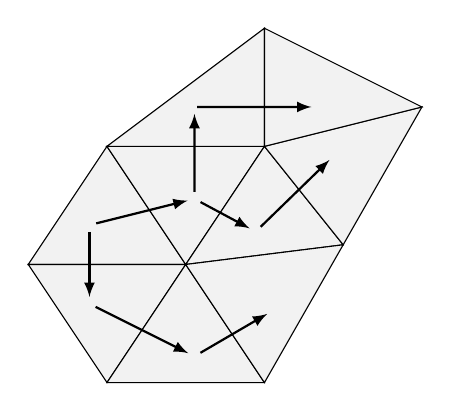
\begin{tikzpicture}
    \coordinate (A) at (0,0);
    \coordinate (B) at (2,0);
    \coordinate (C) at (1,1.5);
    \coordinate (D) at (3,1.5); 
    \coordinate (E) at (3,3); 
    \coordinate (F) at (4,0.25); 
    \coordinate (X) at (1,-1.5);
    \coordinate (Y) at (3,-1.5); 
    \coordinate (T) at (5,2); 
    
    \coordinate (CentroidABC) at ($(A)!0.3333!(B)!0.3333!(C)$);
    \coordinate (CentroidBCD) at ($(B)!0.3333!(C)!0.3333!(D)$);
    \coordinate (CentroidCDE) at ($(C)!0.3333!(D)!0.3333!(E)$);
    \coordinate (CentroidBDF) at ($(B)!0.3333!(D)!0.3333!(F)$);
    \coordinate (CentroidABX) at ($(A)!0.3333!(B)!0.3333!(X)$);
    \coordinate (CentroidBXY) at ($(Y)!0.3333!(B)!0.3333!(X)$);
    \coordinate (CentroidBFY) at ($(Y)!0.3333!(B)!0.3333!(F)$);
    \coordinate (CentroidDFT) at ($(D)!0.3333!(F)!0.3333!(T)$);
    \coordinate (CentroidDET) at ($(D)!0.3333!(E)!0.3333!(T)$);
    
    \draw[fill=gray!10] (A) -- (B) -- (C) -- cycle; 
    \draw[fill=gray!10] (B) -- (C) -- (D) -- cycle; 
    \draw[fill=gray!10] (C) -- (D) -- (E) -- cycle; 
    \draw[fill=gray!10] (B) -- (D) -- (F) -- cycle; 
    \draw[fill=gray!10] (A) -- (B) -- (X) -- cycle; 
    \draw[fill=gray!10] (Y) -- (B) -- (X) -- cycle; 
    \draw[fill=gray!10] (Y) -- (B) -- (F) -- cycle; 
    \draw[fill=gray!10] (T) -- (D) -- (F) -- cycle; 
    \draw[fill=gray!10] (T) -- (D) -- (E) -- cycle; 
    
    \draw[-latex, thick, shorten <=2.5pt, shorten >=2.5pt] (CentroidABC) -- (CentroidBCD); 
    \draw[-latex, thick, shorten <=2.5pt, shorten >=2.5pt] (CentroidBCD) -- (CentroidCDE); 
    \draw[-latex, thick, shorten <=2.5pt, shorten >=2.5pt] (CentroidBCD) -- (CentroidBDF); 
    \draw[-latex, thick, shorten <=2.5pt, shorten >=2.5pt] (CentroidABC) -- (CentroidABX); 
    \draw[-latex, thick, shorten <=2.5pt, shorten >=2.5pt] (CentroidABX) -- (CentroidBXY); 
    \draw[-latex, thick, shorten <=2.5pt, shorten >=2.5pt] (CentroidBXY) -- (CentroidBFY); 
    \draw[-latex, thick, shorten <=2.5pt, shorten >=2.5pt] (CentroidBDF) -- (CentroidDFT); 
    \draw[-latex, thick, shorten <=1.0pt, shorten >=2.0pt] (CentroidCDE) -- (CentroidDET); 
    
%     \node at (A) [below left] {$A$};
%     \node at (B) [below right] {$B$};
%     \node at (C) [above] {$C$};
%     \node at (D) [above right] {$D$};
%     \node at (T) [above right] {$T$};
\end{tikzpicture}
\end{center}
\caption{Strongly connected triangulation of a domain. The arrows depict a tree in the strong connection graph of the form used in Theorem~\ref{theorem:poincarefriedrichsestimate:grad}.}
\end{figure}

\begin{theorem}\label{theorem:poincarefriedrichsestimate:grad}
    Let $\Omega \subseteq \bbR^{n}$ be a domain with a strongly-connected finite triangulation $\calT$.
    Let $T_0 \in \calT$ be an $n$-simplex such that for all $n$-simplices $T \in \calT$ 
    we fix a strong path $T_0, T_1, \dots, T_m = T$.
    Then for any $u \in W^{1,p}(\Omega)$ 
    there exists $w \in W^{1,p}(\Omega)$ with $\nabla u = \nabla w$ 
    and such that for all $T \in \calT$:
    \begin{align*}
        \| w_{m} \|_{L^{p}(T_m)}^{p}
        &\leq 
        (m+1)^{p-1}
        \sum_{t=1}^{m} 
        \left( 
            \prod_{t < l \leq m} 
            \frac{ \vol(T_l) }{ \vol(T_{l-1}) } 
        \right)
        \left( 1 + \frac{ \vol(T_t)^{\frac q p} }{ \vol(T_{t-1})^{\frac q p} } \right)^{p/q}
        C_{p,T_{t} \cup T_{t+1}}
        \| \nabla u \|_{L^{p}( T_{t} \cup T_{t+1} )}^{p}
        \\&\quad \quad \quad 
        +
        (m+1)^{p-1}
        \left( 
            \prod_{0 < l \leq m} 
            \frac{ \vol(T_l) }{ \vol(T_{l-1}) } 
        \right)
        C_{p,T_{0}}
        \| \nabla u \|_{L^{p}(T_{0})}^{p}
        .
    \end{align*}
\end{theorem}

\begin{proof}
 Let $u \in W^{1,p}(\Omega)$. 
 For each $F \in \calT$ of dimension $n-1$, 
 we let $u_F \in W^{1,p}(U_F)$ such that $\nabla u_F = \nabla u$ over $U_F$ and such that $\| u_F \|_{L^{p}(U_F)} \leq C_{{\rm{P}},F,p} \| \nabla u_F \|_{L^{p}(U_F)}$.
 
 There exists $w_0 \in W^{1,p}(T_{0})$ satisfying $\nabla w_0 = \nabla u$ over $T_{0}$ together with 
 \[
    \| w_0 \|_{L^{p}(T_{0})} \leq C_{{\rm{P}},T_{0},p} \| \nabla u \|_{L^{p}(T_{0})}.
 \]
 In particular, $c_{\star} := u - w_0$ is a constant function. 
 Now, let $T \in \calT$ be any $n$-simplex. 
 By assumption, there exists a strong path $T_0, T_1, \dots, T_M = T$, composed of $n$-simplices. 
 For any $1 \leq m \leq M$ we let $F_m := T_m \cap T_{j(m)}$ be a face of dimension $n-1$. 
 We write $\Omega_m := \cup_{j=0}^{m} T_m$, which is a triangulated $n$-dimensional submanifold with boundary.
 
%  Since $\calT$ is strongly connected, there exists an enumeration of $n$-simplices $T_0, T_1, \dots, T_M$ such that for any $1 \leq m \leq M$ there exists some fixed but arbitrary $0 \leq j(m) < m$ such that $F_m := T_m \cap T_{j(m)}$ is a face of dimension $n-1$. We write $\Omega_m := \cup_{j=0}^{m} T_m$. Hence $\Omega = \Omega_M$. 
 
 Suppose that $1 \leq m \leq M$ such that there exists $w_{m-1} \in W^{1,p}(\Omega_{m-1})$ 
 such that $c_{\star} = w_{m-1} - u_{|\Omega_{m-1}}$ is the constant above. 
 Hence $\nabla w_{m-1} = \nabla u$ over $\Omega_m$. 
 By assumption, $T_{m}$ shares the face $F_{m}$ with $T_{{m-1}}$. 
 Since $\nabla u_{F_{m}|T_{{m-1}}} = \nabla w_{m-1|T_{{m-1}}}$,
 there exists a constant $c_{m} := w_{m-1|T_{{m-1}}} - u_{F_{m}|T_{{m-1}}}$.
 We define $w'_{F_m} := u_{F_m} + c_{m} \in W^{1,p}(U_F)$.
 By construction, $\nabla w'_{F_m} = \nabla u_{F_m} = \nabla u_{|U_{F_m}}$ 
 and 
 $w'_{F_{m}|T_{{m-1}}} = w_{m-1|T_{{m-1}}}$. 
 But that already implies $w'_{F_m} = u_{|F_m} - c_{\star}$. 
 We define a measurable function $w_{m} \in W^{1,p}(\Omega_m)$ by extending $w_{m-1}$ with $w'_{F_m|T_m}$.
 We have $c_{\star} = w_{m} - u_{|\Omega_{m}}$. 
 
 We assess the norm of this potential. We observe 
 \begin{gather*}
    \| u'_{F_m} \|_{L^{p}(T_m)}
    \leq 
    \| u_{F_m} \|_{L^{p}(T_m)}
    +
    \| c_{m} \|_{L^{p}(T_m)},
    \qquad 
    \| c_{m} \|_{L^{p}(T_m)}
    \leq 
    \frac{ \vol(T_m)^{\frac 1 p} }{ \vol(T_{{m-1}})^{\frac 1 p} }
    \| c_{m} \|_{L^{p}(T_{{m-1}})},
    \\ 
    \| c_{m} \|_{L^{p}(T_{{m-1}})}
    \leq 
    \| w_{m-1}\|_{L^{p}(T_{{m-1}})} + \| u_{F_{m}} \|_{L^{p}(T_{{m-1}})} 
    .
 \end{gather*}
 In particular,
 \begin{align*}
    \| w_{m} \|_{L^{p}(T_m)}
    \leq 
    \| u_{F_m} \|_{L^{p}(T_m)}
    +
    \frac{ \vol(T_m)^{\frac 1 p} }{ \vol(T_{{m-1}})^{\frac 1 p} }
    \| u_{F_{m}} \|_{L^{p}(T_{{m-1}})}
    +
    \frac{ \vol(T_m)^{\frac 1 p} }{ \vol(T_{{m-1}})^{\frac 1 p} }
    \| w_{m-1}\|_{L^{p}(T_{{m-1}})}
    .
 \end{align*}
 We summarize the two integrals of $u_{F_m}$. 
 % 
 In the special case $p=1$,
 \begin{align*}
    \| w_{m} \|_{L^{1}(T_m)}
    \leq 
    \max\left(
        1, \frac{ \vol(T_m) }{ \vol(T_{{m-1}}) } 
    \right)
    \| u_{F_m} \|_{L^{1}(U_{F_m})}
    +
    \frac{ \vol(T_m) }{ \vol(T_{{m-1}}) }
    \| w_{m-1}\|_{L^{1}(T_{{m-1}})}
    .
 \end{align*}
 In the special case $p=\infty$, 
 \begin{align*}
    \| w_{m} \|_{L^{\infty}(T_m)}
    \leq 
    2
    \| u_{F_m} \|_{L^{\infty}(U_{F_m})}
    +
    \| w_{m-1}\|_{L^{\infty}(T_{{m-1}})}
    .
 \end{align*}
 When $1 < p < \infty$, letting $q$ be the complementary exponent, we observe 
 \begin{align*}
    \| w_{m} \|_{L^{p}(T_m)}
    &\leq 
    \left( 1 + \frac{ \vol(T_m)^{\frac q p} }{ \vol(T_{{m-1}})^{\frac q p} } \right)^{\frac 1 q}
    \left( 
        \| u_{F_m} \|_{L^{p}(T_m)}^{p}
        +
        \| u_{F_{m}} \|_{L^{p}(T_{{m-1}})}^{p}
    \right)^{\frac 1 p}
    +
    \frac{ \vol(T_m)^{\frac 1 p} }{ \vol(T_{{m-1}})^{\frac 1 p} }
    \| w_{m-1}\|_{L^{p}(T_{{m-1}})}
    \\&\leq 
    \left( 1 + \frac{ \vol(T_m)^{\frac q p} }{ \vol(T_{{m-1}})^{\frac q p} } \right)^{\frac 1 q}
    \| u_{F_m} \|_{L^{p}(U_{F_m})} 
    +
    \frac{ \vol(T_m)^{\frac 1 p} }{ \vol(T_{{m-1}})^{\frac 1 p} }
    \| w_{m-1}\|_{L^{p}(T_{{m-1}})}
    .
 \end{align*}
 Recursive application provides the following estimate:
 if $T_0 = S_0, S_1, \dots, S_m = T_m$ is a sequence of $n$-simplices in $\calT$
 such that \color{red}$S_{t-1}$ precedes $S_{t}$ in the graph \color{black} and such that $F_t = S_t \cap S_{t-1}$,
 then 
 \begin{align*}
    \| w_{m} \|_{L^{p}(S_m)}
    &\leq 
    \sum_{t=1}^{m} 
    \left( 
        \prod_{t < l \leq m} 
        \frac{ \vol(S_l)^{\frac 1 p} }{ \vol(S_{l-1})^{\frac 1 p} } 
    \right)
    \left( 1 + \frac{ \vol(S_t)^{\frac q p} }{ \vol(S_{t-1})^{\frac q p} } \right)^{\frac 1 q}
    \| u_{F_t} \|_{L^{p}(U_{F_t})}
    \\&\quad \quad \quad 
    +
    \left( 
        \prod_{0 < l \leq m} 
        \frac{ \vol(S_l)^{\frac 1 p} }{ \vol(S_{l-1})^{\frac 1 p} } 
    \right)
    \| u_{S_0}\|_{L^{p}(S_{0})}
    .
 \end{align*}
 It follows that
 \begin{align*}
    \| w_{m} \|_{L^{p}(S_m)}^{p}
    &\leq 
    (m+1)^{p-1}
    \sum_{t=1}^{m} 
    \left( 
        \prod_{t < l \leq m} 
        \frac{ \vol(S_l) }{ \vol(S_{l-1}) } 
    \right)
    \left( 1 + \frac{ \vol(S_t)^{\frac q p} }{ \vol(S_{t-1})^{\frac q p} } \right)^{p/q}
    \| u_{F_t} \|_{L^{p}(U_{F_t})}^{p}
    \\&\quad \quad \quad 
    +
    (m+1)^{p-1}
    \left( 
        \prod_{0 < l \leq m} 
        \frac{ \vol(S_l) }{ \vol(S_{l-1}) } 
    \right)
    \| u_{S_0}\|_{L^{p}(S_{0})}^{p}
    .
 \end{align*}
 Notice that $p/q = p - 1$.
 
 Repeating this argument produces $w \in L^{p}(\Omega)$ 
 such that for all $n$-simplices $T \in \calT$ we have the restriction $w_{|T} \in W^{1,p}(T)$ with $w_{|T} = u + c_{\star}$.
 In particular, $w \in W^{1,p}(\Omega)$ with $\nabla w = \nabla u$.
\end{proof}

We also want to assess an alternative route towards Poincar\'e--Friedrichs inequalities over triangulated domains,
While the underlying idea remains the same, the construction of the potential is slightly different. 
As an auxiliary result with independent relevance, we compute an upper bound for the Poincar\'e--Friedrichs inequality 
when homogeneous boundary conditions are imposed on a single face of the boundary. 
% Upper bounds for the classical Poincar\'e inequality over a simplex is widely known. 

\begin{lemma}\label{lemma:mixedbconsimplex}
    Let $T$ be an $n$-simplex and with a face $F$. 
    If $u \in W^{1,p}(T)$ such that $\trace_{F} u = 0$, then 
    \begin{align*}
        \| u \|_{L^{p}(T)}
        &
        \leq 
        C_{{\rm PF},T,F,p} \diam(T) \| \nabla u \|_{L^{p}(T)}
    \end{align*}
    where $C_{\partial,p} > 0$ is a constant such that 
    \begin{align*}
        C_{{\rm PF},T,F,p}
        \leq 
        \left( C_{{\rm PF},T,p} + \left( C_{{\rm PF},T,p}^{p} + p \cdot C_{{\rm PF},T,p}^{p-1} \right)^{\frac 1 p} \right),  
        \quad 
        C_{{\rm PF},T,F,p}
        \leq 
        2^{\frac n p}
        .
    \end{align*}
\end{lemma}
\begin{proof}
    There exists $w \in W^{1,p}(T)$ with $\nabla w = \nabla u$ and 
    \[
        \| w \|_{L^{p}(T)}
        \leq 
        C_{{\rm PF},T,p} 
        \| \nabla w \|_{\bfL^{p}(T)}
        .
    \]
    Then $w-u$ is constant, and thus $\gamma := \trace_{F} (w-u) = \trace_{F} w$. 
    We use that 
    \[
        \| \gamma \|_{L^{p}(T)}
        =
        \gamma \vol(T)^\frac{1}{p}
        =
        \left( \frac{ \vol(T) }{ \vol(F) } \right)^\frac{1}{p}
        \cdot 
        \gamma 
        \vol(F)^\frac{1}{p}
        \leq 
        \left( \frac{ \vol(T) }{ \vol(F) } \right)^\frac{1}{p}
        \| \gamma \|_{L^{p}(F)}
        .
    \]
    Using a trace inequality~\cite[Lemma~2.8]{veeser2012poincare} when $1 \leq p < \infty$, we find 
    \begin{align*}
        \| \gamma \|_{L^{p}(F)}^{p}
        &
        \leq 
        \frac{ \vol(F) }{ \vol(T) }
        \| w \|_{L^{p}(T)}^{p}
        +
        p
        \cdot 
        \diam(T)
        \frac{ \vol(F) }{ \vol(T) }
        \| w \|_{L^{p}(T)}^{p-1}
        \| \nabla w \|_{L^{p}(T)}
        \\&
        \leq 
        \left( C_{{\rm PF},T,p}^{p} + p \cdot C_{{\rm PF},T,p}^{p-1} \right) 
        \diam(T)^{p}
        \left( \frac{ \vol(F) }{ \vol(T) } \right)
        \| \nabla w \|_{L^{p}(T)}^{p}
        .
    \end{align*}
    Recall that $u = w - \gamma$. The first inequality follows. 
    
    There exists $\varphi : \hat T \rightarrow T_{m+1}$ mapping the convex closure of the $n$ unit vectors onto the face $F$.
    We let $\hat u := u \circ \varphi$ and define $\hat g \in \bfL^p(\hat T)$ via $\hat g := \nabla ( u \circ \varphi )$. 
    Then $\nabla \hat u = \hat g$. 
    % 
    Let $\hat U$ be the unit ball of the $\ell^1$ metric, which contains $\hat T$.
    We let $\tilde u$ be the extension of $\hat u$ onto $\hat U$ by reflection across the coordinate axes.
    We define $\tilde g = \nabla \tilde u$
    and see that $\tilde g$ is the extension of $\hat g$ onto $\hat U$ by reflection across the coordinate axes. 
    By construction $\tilde u$ vanishes at the boundary of $\hat U$, and thus Friedrichs inequality satisfies 
    \begin{gather*}
        \| \tilde u \|_{L^{p}(\hat U)} 
        \leq 
        2 
        \| \tilde g \|_{\bfL^{p}(\hat U)}
        .
    \end{gather*}
    In addition to that, 
    \begin{gather*}
        \| u \|_{L^{p}(T_{m+1})}
        \leq 
        |\det(\Dif \varphi)|^{\frac 1 p} 
        \| \hat u \|_{L^{p}(\hat T)}
        \leq 
        |\det(\Dif \varphi)|^{\frac 1 p} 
        \| \tilde u \|_{L^{p}(\hat U)}
        ,
        \\
        \| \tilde g \|_{\bfL^{p}(\hat U)}
        \leq 
        2^{\frac n p}
        \| \hat g \|_{\bfL^{p}(\hat T)}
        \leq 
        2^{\frac n p}
        |\det(\Dif \varphi_1)|^{-\frac 1 p} \| \Dif \varphi \| \cdot 
        \| \nabla u \|_{\bfL^{p}(T)}
        .
    \end{gather*}
    The second inequality follows.
\end{proof}

The following potential construction and upper bound for the Poincar\'e--Friedrichs constant 
serves as the blueprint for constructing potentials of the curl and divergence operators in later sections. 

\begin{theorem}\label{theorem:poincarefriedrichsestimate:gradzwei}
    Let $\Omega \subseteq \bbR^{n}$ be a domain with a strongly connected finite triangulation $\calT$.
    Let $T_0 \in \calT$ be an $n$-simplex such that for all $n$-simplices $T \in \calT$ 
    we fix a strong path $T_0, T_1, \dots, T_m = T$.
    Then for any $u \in W^{1,p}(\Omega)$ 
    there exists $w \in W^{1,p}(\Omega)$ with $\nabla u = \nabla w$ 
    and such that for all $T \in \calT$:
    \begin{align*}
        \| w_{m} \|_{L^{p}(T_m)}
        &\leq 
        \sum_{l=1}^{m} 
        \rho(\calT)^{\frac{m-l}{p}}
        C_{{\rm PF},T,p} \left( 1 + \rho(\calT)^{\frac 1 p} \xi(\calT) \right) \diam(T_{0})
        \| \nabla u \|_{L^{p}( T_{l} )}
        +
        \rho(\calT)^{\frac m p}
        C_{{\rm PF},T_{0},p} \diam(T_{0})
        \| \nabla u \|_{L^{p}( T_{0} )}
        .
    \end{align*}
    \color{red}Precise form of the inequality yet to be discussed, though the construction principle is clear.
\end{theorem}

\begin{proof}
    Let $u \in W^{1,p}(\Omega)$. 
    Since $\calT$ is strongly connected, there exists an enumeration of $n$-simplices $T_0, T_1, \dots, T_M$ such that for any $1 \leq m \leq M$ there exists some fixed but arbitrary $0 \leq j(m) < m$ such that $F_m := T_m \cap T_{j(m)}$ is a face of dimension $n-1$. 
    We write $\Omega_m := \cup_{j=0}^{m} T_m$. Hence $\Omega = \Omega_M$. 
    
    First, there exists $w_0 \in W^{1,p}(T_{0})$ such that $\nabla w_{0} = \nabla u$ over $\Omega_0$. 
    Suppose that $0 \leq m < M$ such that there exists $w_{m} \in W^{1,p}(\Omega_{m})$ with $\nabla w_{m} = \nabla u$ over $\Omega_m$. 
    Hence $w_{m} - u_{|\Omega_{m}}$ is a constant. 
    
    By assumption, $T_{m}$ shares the face $F_{m}$ with $T_{j(m)}$. 
    Let $\hat T$ be the reference simplex.
    % We fix affine homeomorphisms $\varphi : \hat T \rightarrow T_{j(m)}$ and $\vartheta : \hat T \rightarrow T_{m+1}$,
    % each of which maps the convex closure of $v_0, \dots, v_{n-1}$ onto the common face $F_{m}$.
    %
    We define $w'_{m+1} := w_{m} \circ \Xi \in W^{1,p}(T_{m+1})$,
    where $\Xi : T_{m+1} \rightarrow T_{j(m)}$ is the unique affine homeomorphism that leaves $F$ invariant. 
    %
    By construction, $w'_{m+1} \in W^{1,p}(T_{m+1})$ with 
    \begin{align*}
        \trace_F w_{m} = \trace_F w'_{m+1}
        .
    \end{align*}
    Suppose that $w''_{m+1} = u - w'_{m+1} \in W^{1,p}(T_{m+1})$.
    It satisfies 
    \begin{align*}
        \nabla w''_{m+1} = \nabla u - \nabla w'_{m+1}, 
        \quad 
        \trace_{F_{m}} w''_{m+1} = 0.
    \end{align*}
    The trace condition holds because 
    \begin{align*}
        \trace_{F_{m}}( \nabla u - \nabla w'_{m+1} ) 
        &= 
        \trace_{F_{m}} \nabla u - \trace_{F_{m}} \nabla w'_{m+1}
        \\&= 
        \nabla \trace_{F_{m}} u - \nabla \trace_{F_{m}} w'_{m+1}
        = 
        \nabla \trace_{F_{m}} u - \nabla \trace_{F_{m}} w_{m}
        = 
        0
        .
    \end{align*}
    Setting $w_{m+1} := w_{m}$ over $\Omega_{m}$ and $w_{m+1} := w'_{m+1} + w''_{m+1}$ over $T_{m+1}$, 
    we find 
    \begin{gather*}
        \nabla w_{m+1} = \nabla w'_{m+1} + \nabla w''_{m+1} = \nabla w'_{m+1} + \nabla u - \nabla w'_{m+1} = \nabla u,
        % \end{gather*}
        \\
        % \begin{gather*}
        \trace_{F_{m}} w_{m+1} = \trace_{F_{m}} w'_{m+1} = \trace_{F_{m}} w_{m}.
    \end{gather*}
    That means that $w_{m+1} \in W^{1,p}(\Omega_{m+1})$ with $\nabla w_{m+1} = \nabla u$ over $\Omega_{m+1}$. 
    Lemma~\ref{lemma:mixedbconsimplex} gives 
    \begin{align*}
        \| w''_{m+1} \|_{L^{p}(T_{m+1})} 
        &
        \leq 
        C_{{\rm PF},T,F,p} \diam(T_{m+1}) \| \nabla u - \nabla w'_{m+1} \|_{L^{p}(T_{m+1})}.
        \\&
        \leq 
        C_{{\rm PF},T,F,p} \diam(T_{m+1}) \| \nabla u        \|_{L^{p}(T_{m+1})} 
        + 
        C_{{\rm PF},T,F,p} \diam(T_{m+1}) \| \nabla w'_{m+1} \|_{L^{p}(T_{m+1})} 
        .
    \end{align*}
    We also employ Lemma~\ref{lemma:volumecomparison} to find 
    \begin{align*}
        \| \nabla w'_{m+1} \|_{L^{p}(T_{m+1})}
        &\leq 
        |\det(\Dif \Xi  )|^{-\frac 1 p} 
        \| \Dif \Xi   \|
        \cdot 
        \| \nabla w_{m} \|_{L^{p}(T_{m})}
        \leq 
        \rho(\calT)^{\frac 1 p} \xi(\calT)
        \cdot 
        \| \nabla w_{m} \|_{L^{p}(T_{m})}
        .
    \end{align*}
    Putting this all together, 
    \begin{align*}
        &
        \| w_{m+1} \|_{L^{p}(T_{m+1})}
        \\&
        \leq  
        \| w'_{m+1} \|_{L^{p}(T_{m+1})}
        + 
        \| w''_{m+1} \|_{L^{p}(T_{m+1})}
        \\&
        \leq  
        \rho(\calT)^{\frac 1 p} 
        \| w_{m} \|_{L^{p}(T_{m})} 
        + 
        C_{{\rm PF},T,F,p} \diam(T_{m+1}) 
        \left( 
            \| \nabla u \|_{L^{p}(T_{m+1})} 
            + 
            \| \nabla w'_{m+1} \|_{L^{p}(T_{m+1})} 
        \right) 
        \\&
        \leq  
        \rho(\calT)^{\frac 1 p} 
        \| w_{m} \|_{L^{p}(T_{m})} 
        + 
        C_{{\rm PF},T,F,p} 
        \left( 1 + \rho(\calT)^{\frac 1 p} \xi(\calT) \right) 
        \diam(T_{m+1}) 
        \| \nabla u \|_{L^{p}(T_{m+1})} 
        .
    \end{align*}
    The recursive estimate follows. 
\end{proof}

\begin{remark}
    The previous theorems, Theorem~\ref{theorem:poincarefriedrichsestimate:gradzwei} and Theorem~\ref{theorem:poincarefriedrichsestimate:gradzwei} 
    depend on only a few parameters of the triangulation:
    the length of any traversal from the root simplex, the ratios of the volumes of adjacent simplices,
    the Poincar\'e constants on each face patch, and the Poincar\'e constant of the initial simplex. 
    The aforementioned local Poincar\'e constants can generally be estimated in terms of shape-parameters. 
    If the face patches of the triangulation are convex, then better estimates are possible. 
\end{remark}

% https://people.tamu.edu/~guermond//PUBLICATIONS/ern_guermond_m2an_2016.pdf 
% Lemma 5.5























\section{Shellable triangulations}\label{section:advancedtriangulations}

We return to the theory of triangulations,
as our main objective requires some further concepts.
We are interested in simplicial complexes that triangulated manifolds. 
We put particular focus on \emph{shellable} simplicial complexes as a particularly important class of complexes. Such simplicial complexes are constructed by successively adding simplices in a particularly well-behaved manner. Patches within triangulations are examples of such shellable complexes. 
Our main references for this section are the monographs by Kozlov~\cite{kozlov2008combinatorial} and Ziegler~\cite{ziegler2012lectures}. 

\begin{remark}
It is often very helpful if a simplicial complex can be created recursively, starting with a single simplex. In particular, this enables the inductive method of proof.
Formally, a triangulation is shellable if its full-dimensional simplices can be enumerated such that each simplex intersects the union of the previously listed simplices in a codimension one triangulation. 
Roughly speaking, a triangulation is shellable if the triangulation can be built, starting from a single simplex,
by successively gluing simplices to intermediate triangulations such that a combinatorial-geometric condition is satisfied:
the gluing interface is a triangulated submanifold of the boundary. 
This forces the intermediate triangulations to be particularly well-shaped. 
\end{remark}

\subsection{Triangulations of manifolds}

We define an $n$-dimensional simplicial complex to be a \emph{manifold triangulation} if the underlying set $\underlying{\calT}$ is an $n$-dimensional manifold with boundary.
We recall that this means that for every $x \in \underlying{\calT}$
there exists $\epsilon > 0$ and an embedding $\phi : \Ball_\epsilon(x) \cap \underlying{\calT} \rightarrow \bbR^{n}$
such that $\phi(0) = 0$ and $\phi$ is an isomorphism either onto the closed unit ball $\calB = \{ x \in \bbR^{n} \suchthat |x| \leq 1 \}$
or onto $\{ x \in \calB \suchthat x_1 \geq 0 \}$.
Any simplicial complex that triangulates an $n$-dimensional manifold must be $n$-dimensional.

We know that any manifold $\calM$ has a got a topological boundary $\partial\calM$, possibly empty. 
If $\calM$ is $n$-dimensional, then the $\partial\calM$ is a topological manifold without boundary of dimension $n-1$. 

The following special cases receive particular interest:
a \textit{$n$-ball triangulation} is any triangulation of a topological (closed) $n$-ball,
and we sometimes call this a \textit{$n$-disk} triangulation.
An \textit{$n$-sphere triangulation} is any triangulation of a topological $n$-sphere. 

We gather a few helpful properties of manifold triangulations. 
While the reader might deem them obvious, we nevertheless include proofs. 
We begin with the boundary.

\begin{lemma}\label{lemma:boundarysimplices}
    Let $\calT$ be a finite $n$-dimensional simplicial complex whose underlying space is a manifold $\calM$. 
    \begin{itemize}
        \item Any face $F \in \Faces(\calT)$ is not contained in the boundary if and only if it is contained in exactly two $n$-simplices.
        \item Any face $F \in \Faces(\calT)$ is contained in the boundary if and only if it is contained in exactly one $n$-simplex.
        \item The simplices contained in the boundary constitute a triangulation of the boundary.
        % \item $\calT$ is non-branching, that is, every $F \in \calT$ of dimension $n-1$ is contained in at most two $n$-simplices of $\calT$. 
    \end{itemize}
\end{lemma}
\begin{proof}
    We prove these statements in several steps.
    \begin{enumerate}
    \item 
    We $\mathring \calM := \calM \setminus \partial \calM$ denote the interior of the manifold. 
    We will use the following fact: if $S \in \calT$ has an inner point that lies on $\partial \calM$, then all inner points of $S$ are on $\partial \calM$. 
    Since the boundary is closed, every $S \in \calT$ is either a subset of the boundary or all its inner points lie in the interior $\mathring \calM$ of the manifold. 
    
    \item
    Let $F \in \Faces(T)$ and let $z_F \in F$ be its midpoint. 
    Let $\mathring B_F$ be an open neighborhood around $z_F$ so small that it only intersects those $n$-simplices of $\calT$ that already contain $z_F$ and no faces other than $F$.
    Suppose there are distinct $n$-simplices $T_1, T_2, \dots, T_K$ that contain $z_F$. 
    The intersection of any two of them is $F$, and their interiors are disjoint. 
    
    If $z_F$ is an interior point of $\calM$, 
    then we can assume that $\mathring B_F$ is homeomorphic to an open $n$-ball and $\partial \mathring B_F$ is homeomorphic to a sphere $S$ of dimension $n-1$. 
    At the same time, $X = F \subseteq \partial \mathring B_F$ is empty if $n=1$ or homeomorphic to a sphere $S' \subseteq S$ of dimension $n-2$. 
    We see that $\partial \mathring B_F \setminus X$ has $K$ distinct connected components. 
    But by construction $\partial \mathring B_F \setminus X$ is homeomorphic to $S \setminus S'$,
    which has exactly two distinct connected components according to the Jordan-Brouwer separation theorem.
    We conclude that $F$ is contained in two $n$-simplices of $\calT$.
    If an inner face $F$ were contained in only one $n$-simplex,
    then we could construct a homeomorphism from the $n$-ball onto itself that maps an interior point on the its boundary, which cannot be.
    So each inner face is contained in exactly two $n$-simplices. 
    
    If $F$ is contained in only one $n$-simplex, then it must be a face in the boundary of $\calM$. 
    If $F$ were contained in at least two $n$-simplices,
    then we could construct a homeomorphism from the $n$-ball onto itself that maps an interior point on the its boundary, which cannot be.
    So each face within $\partial \calM$ is contained in exactly one $n$-simplex. 
    
    \item
    Clearly, the simplices of $\calT$ contained in the boundary constitute a simplicial complex. 
    If $x \in \partial \calM$ is a boundary simplex, then it is an inner point of some simplex $S \in \calT$.
    But then this simplex must be a boundary simplex, so the boundary simplices form a triangulation of $\partial \calM$.
    \end{enumerate}
    All relevant results are proven. 
\end{proof}

%%%%%%%%%%%%%%%%%%%%%%%%%%%%%%%%%% TODO: integrate into narrative 
Suppose that $\calT$ is an $n$-dimensional simplicial complex that triangulates a manifold. 
Those simplices of the manifold triangulation that are subsets of the boundary of the underlying manifold are called \emph{boundary simplices}. 
% The simplices that lie in the boundary of the underlying set are called \emph{boundary simplices}.
All other simplices of the manifold triangulation are called \emph{inner simplices}. 

We have seen that the boundary simplices of a manifold triangulation constitute a triangulation of the manifolds boundary. 
We call this simplicial complex the \emph{boundary complex}. It has dimension $n-1$. 
% We see that the family of boundary faces constitute a simplicial complex, which we call \textit{boundary complex}.
% Any point on the boundary lies within some boundary simplex, and hence the boundary complex is a triangulation of the boundary. 
% Definitions imply that the boundary complex is a manifold triangulation of dimension $n-1$.
% The boundary simplices of a manifold triangulation of dimension $n$ constitute a manifold triangulation themselves, of dimension $n-1$, which triangulate the boundary of the underlying space. 
%%%%%%%%%%%%%%%%%%%%%%%%%%%%%%%%%%%
\\

We continue with a few more observations about manifold triangulations.

\begin{lemma}\label{lemma:startopology}
    Let $\calT$ be a finite $n$-dimensional simplicial complex whose underlying space is a manifold $\calM$. 
    \begin{itemize}
        \item If $S$ is an inner simplex, then $\patch_{\calT}(S)$ is a simplicial $n$-ball with $S$ as an inner simplex
        and $\carapace_{\calT}(S)$ is a simplicial $(n-1)$-sphere. 
        \item If $S$ is a boundary subsimplex, then $\patch_{\calT}(S)$ is a simplicial $n$-ball with $S$ as a boundary simplex,
        and $\carapace_{\calT}(S)$ is a simplicial $(n-1)$-ball.
        \item If the underlying space of $\calT$ is connected, then $\calT$ is strongly connected.
    \end{itemize}
\end{lemma}
\begin{proof}
    We prove these statements in several steps.
    \begin{enumerate}
    \item 
    Let $S$ be any simplex with vertices $v_0, v_1, \dots, v_k$, with midpoint $z_F$, and dimension $k$.
    Let $\calS := \patch_{\calT}(S)$ be its star. 
    Each $l$-dimensional simplex $T \in \calS$ that contains $S$ 
    has vertices $v_0, v_1, \dots, v_k, v_{k+1}^{S}, \dots, v_{l}^{S}$. 
    For any such simplex, we introduce a decomposition $T_{0}, \dots, T_{k}$, where each $T_{i}$ has vertices 
    \begin{align*}
        v_0, \dots, v_{i-1}, z_F, v_{i+1}, \dots, v_k, v_{k+1}^{S}, \dots, v_{l}^{S}.
    \end{align*}
    The collection $\calS'$ of these simplices and their subsimplices constitute a simplicial complex 
    that triangulates the same underlying set as $\calS$.
    Moreover, $\calS' = \patch_{\calS'}(z_F)$. 
    In particular, $z_F$ is a boundary vertex of $\calS'$ if and only if $S$ is a boundary simplex of $\calS$. 
    
    So it remains to study the topology of vertex stars. Suppose that $S = \{z\}$ is a singleton simplex. 
    For $\delta > 0$ small enough, 
    \begin{align*}
        B_{\delta}(z) = \left\{ x \in \calM \suchthat d(x,z) \leq \delta \right\},
        \quad 
        S_{\delta}(z) = \left\{ x \in \calM \suchthat d(x,z) = \delta \right\},
    \end{align*}
    are subsets of $\patch_{\calT}(S)$.
    For each $K \in \patch_{\calT}(S)$ that contains $S$ and which has the complementary simplex $F_S$, 
    we easily find homeomorphisms $\phi_{K} : B_{\delta}(z) \cap K \rightarrow K$
    such that 
    $\phi_{K|S}$ is the identity,
    such that 
    $\phi_{K}(S_F) = S_{\delta}(z)$,
    and such that 
    for all $K, K' \in \calT$ with $K' \subseteq K$ we have $\phi_{K|K'} = \phi_{K'}$. 
    
    If $z$ is an inner vertex of $\calS'$, 
    then the boundary simplices of $\calS'$,
    which are the boundary simplices of $\calS$, triangulate a topological sphere of dimension $n-1$.
    
    If $z$ is a boundary vertex of $\calS'$,
    which is the case if and only if $S$ is a boundary simplex, 
    then the underlying space of $\carapace(S)$ is homeomorphic to $S_{\delta}(z)$, 
    which is a topological ball of dimension $n-1$. % TODO: explain why
    
    \item 
    We show that each vertex star is strongly connected via a short induction argument.
    Clearly, any simplicial $1$-ball and simplicial $1$-sphere is strongly connected. 
    Now, if $n \geq 1$, then any vertex star in an $(n+1)$-dimensional manifold triangulation is strongly connected if all simplicial $n$-balls and $n$-spheres are strongly connected.
    The induction argument implies that each vertex star in $\calT$ is strongly connected.

    \item 
    If the underlying space is connected, then we easily see that the underlying space of the $1$-skeleton is path-connected.
    Given $n$-simplices $S,S' \in \calT$, 
    we can thus choose a sequence of $\hat S_0=S,\hat S_1,\dots,\hat S_m=S' \in \calT$ such that $\hat S_{i} \cap \hat S_{i-1} \neq \emptyset$ for all $1 \leq i \leq m$.
    We also notice that each vertex star is strongly connected. 
    We can thus construct change the first sequence to another $S_0=S,S_1,\dots,S'=S_m \in \calT$ 
    such that $S_{i} \cap S_{i-1}$ is a face of both $S_{i}$ and $S_{i-1}$ for all $1 \leq i \leq m$.
    \end{enumerate}
    All relevant results are proven. 
\end{proof}




% TODO: https://arxiv.org/html/1607.08163v3
% https://mathoverflow.net/questions/403415/properties-a-triangulation-must-have-in-order-to-describe-a-manifold





\begin{remark}
    Clearly, not every simplicial complex is the triangulation of some (embedded) topological manifold with or without boundary. 
    Whether a simplicial complex is the triangulation of a manifold is algorithmically undecidable. 
    We therefore are not in pursuit of any easy combinatorial property that indicates whether a simplicial complex (without any further specific assumptions) triangulates a manifold.

    Conversely, not all topological manifolds, even if compact, can be described as a triangulation. 
    Such manifolds appear in dimension four and higher:
    one example is the E8 manifold, which is a compact simply-connected topological $4$-manifold that is homeomorphic to the underlying set of any simplicial complex. The construction of such counterexamples typically involves an infinite procedure.
%     For each dimension $n \geq 5$ there exists an $n$-dimensional compact topological manifold without a triangulation. 
\end{remark}







\begin{figure}
    \centering
    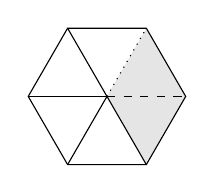
\begin{tikzpicture}
        \coordinate (O) at (0, 0);
        \coordinate (A) at ({cos(0)}, {sin(0)});
        \coordinate (B) at ({cos(60)}, {sin(60)});
        \coordinate (C) at ({cos(120)}, {sin(120)});
        \coordinate (D) at ({cos(180)}, {sin(180)});
        \coordinate (E) at ({cos(240)}, {sin(240)});
        \coordinate (F) at ({cos(300)}, {sin(300)});
        \fill[gray!20] (A) -- (B) -- (O) -- (F) -- cycle;
        \draw (A) -- (B) -- (C) -- (D) -- (E) -- (F) -- cycle;
        \draw[dashed] (O) -- (A); \draw[dotted] (O) -- (B); \draw (O) -- (C); \draw (O) -- (D); \draw (O) -- (E); \draw (O) -- (F);
    \end{tikzpicture}
    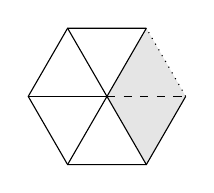
\begin{tikzpicture}
        \coordinate (O) at (0, 0);
        \coordinate (A) at ({cos(0)}, {sin(0)});
        \coordinate (B) at ({cos(60)}, {sin(60)});
        \coordinate (C) at ({cos(120)}, {sin(120)});
        \coordinate (D) at ({cos(180)}, {sin(180)});
        \coordinate (E) at ({cos(240)}, {sin(240)});
        \coordinate (F) at ({cos(300)}, {sin(300)});
        \fill[gray!20] (A) -- (B) -- (O) -- (F) -- cycle;
        \draw[dotted] (A) -- (B); \draw (B) -- (C) -- (D) -- (E) -- (F) -- (A);
        \draw[dashed] (O) -- (A); \draw (O) -- (B); \draw (O) -- (C); \draw (O) -- (D); \draw (O) -- (E); \draw (O) -- (F);
    \end{tikzpicture}
    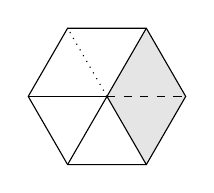
\begin{tikzpicture}
        \coordinate (O) at (0, 0);
        \coordinate (A) at ({cos(0)}, {sin(0)});
        \coordinate (B) at ({cos(60)}, {sin(60)});
        \coordinate (C) at ({cos(120)}, {sin(120)});
        \coordinate (D) at ({cos(180)}, {sin(180)});
        \coordinate (E) at ({cos(240)}, {sin(240)});
        \coordinate (F) at ({cos(300)}, {sin(300)});
        \fill[gray!20] (A) -- (B) -- (O) -- (F) -- cycle;
        \draw (A) -- (B) -- (C) -- (D) -- (E) -- (F) -- cycle;
        \draw[dashed] (O) -- (A); \draw (O) -- (B); \draw[dotted] (O) -- (C); \draw (O) -- (D); \draw (O) -- (E); \draw (O) -- (F);
    \end{tikzpicture}
    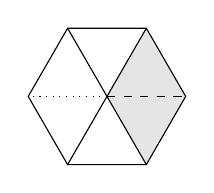
\begin{tikzpicture}
        \coordinate (O) at (0, 0);
        \coordinate (A) at ({cos(0)}, {sin(0)});
        \coordinate (B) at ({cos(60)}, {sin(60)});
        \coordinate (C) at ({cos(120)}, {sin(120)});
        \coordinate (D) at ({cos(180)}, {sin(180)});
        \coordinate (E) at ({cos(240)}, {sin(240)});
        \coordinate (F) at ({cos(300)}, {sin(300)});
        \fill[gray!20] (A) -- (B) -- (O) -- (F) -- cycle;
        \draw (A) -- (B) -- (C) -- (D) -- (E) -- (F) -- cycle;
        \draw[dashed] (O) -- (A); \draw (O) -- (B); \draw (O) -- (C); \draw[dotted] (O) -- (D); \draw (O) -- (E); \draw (O) -- (F);
    \end{tikzpicture}
    \caption{Examples and counterexamples for building a manifold-like $1$-patching of a $2$-dimensional manifold-like triangulation. (1) We have already added the edge patch along the dashed line and we add the edge patch along the dotted line. (2) The new edge patch may already be a subset of the subtriangulation (3) An inadmissible choice because new edge patch has no overlap with current subtriangulation, though the next subtriangulation would be manifold-like (4) An inadmissible choice because new edge patch has no overlap with current subtriangulation and the next subtriangulation would not be manifold-like.}\label{figure:illustrationpatching}
\end{figure}

\begin{figure}
    \centering
    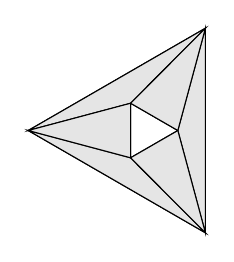
\begin{tikzpicture}[scale=0.5]
        \coordinate (O) at (0, 0);
        \coordinate (A) at ({0.8*cos(  0)}, {0.8*sin(  0)});
        \coordinate (B) at ({0.8*cos(120)}, {0.8*sin(120)});
        \coordinate (C) at ({0.8*cos(240)}, {0.8*sin(240)});
        \coordinate (X) at ({3.0*cos( 60)}, {3.0*sin( 60)});
        \coordinate (Y) at ({3.0*cos(180)}, {3.0*sin(180)});
        \coordinate (Z) at ({3.0*cos(300)}, {3.0*sin(300)});
        \draw (A) -- (B) -- (C) -- cycle; \draw (X) -- (Y) -- (Z) -- cycle;
        \draw[fill=gray!20] (X) -- (Y) -- (B) -- cycle;
        \draw[fill=gray!20] (Y) -- (Z) -- (C) -- cycle;
        \draw[fill=gray!20] (Z) -- (X) -- (A) -- cycle;
        \draw[fill=gray!20] (A) -- (X) -- (B) -- cycle;
        \draw[fill=gray!20] (B) -- (Y) -- (C) -- cycle;
        \draw[fill=gray!20] (C) -- (Z) -- (A) -- cycle;
    \end{tikzpicture}
    \begin{tikzpicture}[scale=0.5]
        \coordinate (O) at (0, 0);
        \coordinate (A) at ({3.0*cos(  0)}, {3.0*sin(  0)});
        \coordinate (B) at ({3.0*cos(120)}, {3.0*sin(120)});
        \coordinate (C) at ({3.0*cos(240)}, {3.0*sin(240)});
        \coordinate (X) at ({3.0*cos( 60)}, {3.0*sin( 60)});
        \coordinate (Y) at ({3.0*cos(180)}, {3.0*sin(180)});
        \coordinate (Z) at ({3.0*cos(300)}, {3.0*sin(300)});
        \draw (O) -- (A);
        \draw (O) -- (B);
        \draw (O) -- (C);
        \draw (O) -- (X);
        \draw (O) -- (Y);
        \draw (O) -- (Z);
        %
    \end{tikzpicture}
    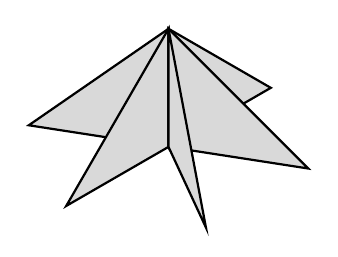
\begin{tikzpicture}[scale=0.5] 
        \tikzset{z={(90:1cm)}, y={(-30:1cm)}, x={(210:1cm)}}
        % \tikzset{z={(90:1cm)}, y={(-10:1cm)}, x={(250:1cm)}}

        \coordinate (O) at (0, 0);
        \coordinate (A) at ({3.0*cos(  0)}, {3.0*sin(  0)});
        \coordinate (B) at ({3.0*cos(120)}, {3.0*sin(120)});
        \coordinate (C) at ({3.0*cos(240)}, {3.0*sin(240)});
        \coordinate (X) at ({3.0*cos( 60)}, {3.0*sin( 60)});
        \coordinate (Y) at ({3.0*cos(180)}, {3.0*sin(180)});
        \coordinate (Z) at ({3.0*cos(300)}, {3.0*sin(300)});
        \coordinate (T) at ({0}, {0}, {3});

        \draw[thick, fill=gray!30] (O) -- (C) -- (T) -- cycle;
        \draw[thick, fill=gray!30] (O) -- (Y) -- (T) -- cycle;
        \draw[thick, fill=gray!30] (O) -- (Z) -- (T) -- cycle;
        \draw[thick, fill=gray!30] (O) -- (A) -- (T) -- cycle;
        \draw[thick, fill=gray!30] (O) -- (B) -- (T) -- cycle;
        \draw[thick, fill=gray!30] (O) -- (X) -- (T) -- cycle;
        
        
    \end{tikzpicture}

    \caption{Example of a connected $2$-dimensional manifold triangulation, which triangulates an annulus, that does neither admit a manifold-like $0$-patching nor manifold-like $1$-patching.}\label{figure:annuluscounterexample}
\end{figure}







% 3. Shellability 
\subsection{Shellable simplicial complexes}

We turn our attention to a different idea of how to incrementally construct a simplicial complex while maintaining well-behaved intermediate complexes. 
We build upon the notion of shelling, as introduced in~\cite[Definition 8.1]{ziegler2012lectures}.
Our definition of shelling is equivalent to the notion of the shellings of simplicial complexes in the aforementioned reference; see also~\cite[Remark~8.3]{ziegler2012lectures}. 

Suppose that $\calT$ is an $n$-dimensional simplicial complex and we have an enumeration of the $n$-simplices $T_{0}, T_{1}, T_{2}, \dots \in \subsimplex_{n}(\calT)$.
For any enumeration, we call 
\begin{align*}
    I_m 
    := 
    \big( 
        T_{0} \cup T_{1} \cup \dots \cup T_{m} 
    \big) 
    \cap 
    T_{m+1}
\end{align*}
be the $m$-th \textit{interface set}. 
% Note that this intersection is automatically a subcomplex of the boundary complex of the last simplex $T_{m}$.
We call the enumeration a \emph{shelling} if each interface $I_m$ is a manifold of dimension $n-1$. 

\begin{remark}
    We interpret a shelling as the construction of a triangulation 
    by successively attaching simplices such that the intermediate triangulations are well-behaved. 
    Conversely, the reverse enumeration describes a successive decomposition of the triangulation, hence the name ``shelling''.
\end{remark}
\begin{remark}
    Whether a simplicial complex is shellable can be checked, in principle, simply by trying out all the possibly enumerations.
    That we cannot do much better than this is captured in the result that testing for shellability is NP-complete~\cite{goaoc2019shellability}:
    this complexity result is even true if we merely consider simplicial complexes of dimension two embedded in some Euclidean space.
\end{remark}




The reason of our interest in shellable simplicial complexes is that they can be constructed by successive adhesion of simplices to intermediate complexes, 
such that the interface is well-behaved: it is a simplicial disk or a simplicial sphere. 
That leads to the following important consequence.

% TODO: we only need some basic properties, namely that the construction maintains manifolds with boundary.
% TODO: copy and adapt the content of Ziegler and Kozlov as necessary
% The notion of shelling is taken from Ziegler's book~\cite{ziegler2012lectures}

\begin{lemma}    
    If an $n$-dimensional simplicial complex $\calT$ has a shelling $T_{0}, T_{1}, T_{2}, \dots, T_{M}$ and is non-branching, 
    then
    $$
        X_{m} := T_{0} \cup T_{1} \cup \dots \cup T_{m}
    $$ 
    is a manifold with boundary for all $0 \leq m \geq M$.
    % 
    In particular, $X_{m}$ is a topological $n$-ball when $m < M$, 
    and 
    $X_{M}$ is either a topological $n$-ball or topological $n$-sphere. 
\end{lemma}
\begin{proof}  
    We prove this claim by induction. 
    Certainly, if $\calT$ contains only one single $n$-simplex, then it is a shellable triangulation of a topological $n$-ball. 
    Suppose that $X_m := T_{0} \cup T_{1} \cup \dots \cup T_{m}$ is a topological $n$-ball and that $T_{m+1}$ is the next $n$-simplex in the shelling.
    By definition, $I_{m+1} := X_{m} \cap T_{m+1}$ is a submanifold of $\partial T_{m+1}$,
    and it is triangulated by some faces of $T_{m+1}$ and their subsimplices. 
    
    Let $F$ be such a face. 
    By assumption, $F$ must be contained in exactly one $n$-simplex of $T_{0}, T_{1}, \dots, T_{m}$,
    and $F$ is in the boundary of $X_{m}$. We conclude that $I_{m}$ triangulates a submanifold of the boundary of $X_{m}$.
    
    On the one hand, 
    if $I_{m+1}$ is the entire boundary of $T_{m+1}$, 
    then it must also be the boundary of the topological $n$-ball $X_{m}$. 
    Hence $X_{m} \cup T_{m+1}$ must be a topological $n$-sphere and thus a manifold without boundary, which requires $m = M$.
    On the other hand, 
    if $I_{m+1}$ is a proper subset of the entire boundary of $T_{m+1}$, 
    then $X_{m} \cup T_{m+1}$ is still a topological $n$-ball.
\end{proof}






We collect important examples of shellable triangulations.
Our main interest are local patches or stars within triangulations. 

\begin{example}
    Any simplex $T$ trivially has a shelling. The boundary complex $\partial \calT(T)$ has a shelling:
    in fact, any enumeration of the boundary faces of $T$ constitutes a shelling.
\end{example}
\begin{example}
    The standard triangulation of the $n$-dimensional cube, the Kuhn triangulation, is shellable. 
    % https://scholar.google.de/scholar?hl=de&as_sdt=0%2C5&q=kuhn+triangulation+shelling&btnG=
\end{example}

\begin{lemma}    
    Any simplicial $2$-disk is shellable.
    Any simplicial $2$-sphere is shellable. 
\end{lemma}
\begin{proof}
    First, 
    let $\calS$ be any triangulation of a $2$-sphere. 
    By removing any triangle $S \in \calS$, we obtain a triangulation $\calT$ of a $2$-disk.
    Any shelling of that disk can be extended to a shelling of $\calS$ by re-inserting the first triangle $S$.
    So it remains to show that any triangulation $\calT$ of the two-dimensional disk is shellable. 
    We will construct the shelling in reverse. 
    
    Write $M = |\calT|$. 
    We call a triangle $T \in \calT$ \emph{good} if it intersects the boundary $\partial M$ in a non-empty union of edges. 
    We show by an induction argument over the number of triangles that every triangulation of a $2$-disk contains a good triangle. 
    Clearly, this is the case if the triangulation contains only one triangle. 
    Now suppose the induction claim is true when the triangulation includes $N$ triangles,
    and assume that $\calT$ includes $N+1$ triangles. 
    There exists a triangle $T' \in \calT$ with at least one edge in the boundary. 
    If $T'$ is good, then we are already done. 
    Otherwise, $T'$ intersects the boundary at one edge and its opposing vertex.
    Removing $T'$ splits the manifold into two pieces, each of which is a topological $2$-disk.
    By the induction assumption, they contain a good triangle.
    
    Since $\calT$ triangulates a $2$-disk,
    it contains a good triangle $T$. 
    If $T$ has three edges in the boundary, then $T = M$ and we are trivially done. 
    If $T$ intersects with the boundary in exactly one or two edges, 
    then $\overline{M \setminus T}$ is still a topological $2$-disk.
    Letting $\calT'$ be the triangulation obtained by removing $T$,
    we have another triangulation of the $2$-disk that intersects $T$ only at either two or one edges.
    Any shelling of $\calT'$ can be extended to a shelling of $\calT$.
%     Let $\calT$ be a simplicial $2$-disk. 
%     If $\calT$ contains only one triangle, then there is nothing to show. 
%     Otherwise, there exists at least one triangle $T$ that touches the boundary of the disk at either one or two edges 
%     {\color{red}Needs proof}. 
%   
%     Now let $\calS$ be any simplicial $2$-sphere. 
%     By removing any triangle $S \in \calS$, we obtain a simplicial $2$-disk, which is shellable. 
%     Any of its shellings can be extended to a shelling of $\calS$ by re-inserting the first triangle $S$.
\end{proof}

% TODO: Ziegler, Lemma 8.7: if a complex has a shelling, then this gives a shelling of the stars 

\begin{lemma}
    Let $\calT$ be a $n$-dimensional manifold triangulation and $V \in \Vertices(\calT)$ be an inner vertex.
    Then $\patch_{\calT}(V)$ is shellable. 
\end{lemma}
\begin{proof}
    Without loss of generality, $V$ is the origin. 
    Any ray starting at $V$ intersects at most one vertex of $\patch_{\calT}(V)$.
    We can also assume that all boundary vertices of $\patch_{\calT}(V)$ to be unit vectors,
    which does not affect shellability. 
    The simplicial boundary complex of $\calT$ is the boundary complex of a convex polytope,
    and is thus shellable~\cite{ziegler2012lectures}. % TODO: cite exactly 
\end{proof}


\begin{lemma}
    Let $\calT$ be a $3$-dimensional manifold triangulation and $S \in \calT$.
    Then $\patch_{\calT}(S)$ is shellable. 
\end{lemma}
\begin{proof}
    The statement is clear if $S$ is an inner or boundary face of $\calT$. 
    The statement is also easily verified if $S$ is an inner or boundary edge of $\calT$.
    When $S$ is an inner vertex, then we apply the preceding lemma. 
    
    It remains to consider the case where $S$ is a boundary vertex. 
    Then the triangles of $\patch_{\calT}(S)$ that do not contain $V$ constitute a simplicial $2$-disk 
    which is shellable,
    and any such shelling can be extended to a shelling of $\patch_{\calT}(S)$.
\end{proof}


\begin{remark}
    Not all trianguable sets admit a triangulation that is also shellable. 
    Moreover, even if a set admits a shellable triangulation, not all of its triangulations might be shellable. 
    We refer to~\cite[Example 8.9]{ziegler2012lectures} for an examples of non-shellable triangulations of cubes and tetrahedra in three dimensions. 

    For example, there exists a non-shellable triangulation of a tetrahedron. 
    If we extend this triangulation to a triangulation of a hypertetrahedron by suspending it from a new point $v_\star$, 
    then the resulting new triangulation is non-shellable and coincides with the patch around $v_\star$.
    This demonstrates that patches around boundary simplices are not necessarily shellable when the dimension exceeds $3$.
\end{remark}


\newpage 








\section{Review of vector calculus and exterior calculus}\label{section:calculus}

We discuss the Sobolev spaces of vector calculus and their transformation behavior. 
Let $\Omega \subseteq \bbR^{3}$ be a bounded open set. 
First, recall that $L^{p}(\Omega)$ is the space of scalar-valued $p$-integrable functions defined on $\Omega$
and that $\bfL^{p}(\Omega) := L^{p}(\Omega)^{n}$ for vector-valued functions with each component in $L^{p}(\Omega)$. 
In the three-dimensional setting, we are particularly interested in the Sobolev vector analysis. 
$W^p(\grad,\Omega) := W^{1,p}(\Omega)$ is the space of scalar-valued $L^{p}(\Omega)$ functions with weak gradients in $\bfL^{p}(\Omega)$, that is,  
\[
    W^p(\grad,\Omega) = \{ u \in L^{p}(\Omega) \suchthat \grad v \in \bfL^{p}(\Omega) \}
\]
The space $\bfW^{p}(\curl,\Omega)$ of vector-valued $\bfL^{p}(\Omega)$ functions with weak curls in $\bfL^{p}(\Omega)$
and the space of vector-valued $\bfL^{p}(\Omega)$ functions with weak divergences in $L^{p}(\Omega)$ are defined as 
\[
    \bfW^{p}(\curl,\Omega) = \{ \bfu \in \bfL^{p}(\Omega) \suchthat \curl \bfu \in \bfL^{p}(\Omega) \},
    \quad 
    \bfW^{p}(\divergence,\Omega) = \{ \bfu \in \bfL^{p}(\Omega) \suchthat \divergence \bfu \in L^{p}(\Omega) \}.
\]
We are interested in transformations of these Sobolev tensor fields from one domain onto the other. 
Suppose that $\Omega, \Omega' \subset \mathbb{R}^3$ are open sets and suppose that $\phi: \Omega \to \Omega'$ is a bi-Lipschitz mapping.
The gradient-, curl-, divergence-conforming Piola transformations are the mappings 
$\phi^{\grad}: L^{p}(\Omega') \to L^{p}(\Omega)$,
$\phi^{\curl}: \bfL^{p}(\Omega') \to \bfL^{p}(\Omega)$, 
$\phi^{\divergence}: \bfL^{p}(\Omega') \to \bfL^{p}(\Omega)$,
and
$\phi^{\rm b}: L^{p}(\Omega') \to L^{p}(\Omega)$. 
They are defined by 
\begin{subequations}\label{eq_definition_piola}
\begin{align}
    \phi^{\grad}(v) &= v \circ \phi, \\
    \phi^{\curl}(\bfw) &= (\Jacobian\phi^{T} \bfw) \circ \phi, \\
    \phi^{\divergence}(\bfw) &= \left( \det(\Jacobian\phi) \Jacobian\phi^{-1} \bfw \right)  \circ \phi, \\
    \phi^{\rm b}(v) &= \left( \det\Jacobian\phi^{-1} v \right)  \circ \phi,
\end{align}
\end{subequations}
where $v \in L^{p}(\Omega')$ and $\bfw \in \bfL^{p}(\Omega')$, 
and where $\Jacobian\phi$ is the Jacobian matrix of $\phi$. 
These mappings are invertible. 
%
% TODO: bounds
%
We use the commutativity relations 
\begin{subequations}\label{eq_piola_commute}
\begin{align}
    \grad (\phi^{\grad} (v)) &= \phi^{\curl}(\grad v), 
    \\
    \curl (\phi^{\curl}(\bfv)) &= \phi^{\divergence}(\curl \bfv) 
    % TODO: watch the sign 
    \\
    \divergence (\phi^{\divergence}(\bfw)) &= \phi^{\rm b}(\divergence \bfw)
\end{align}
\end{subequations}
for $v \in W^{p}(\grad,\Omega)$, $\bfv \in \bfW^{p}(\curl,\Omega)$, and $\bfw \in \bfW^{p}(\divergence,\Omega)$.  
We summarize this as a commuting diagram:
\begin{align*}
    \begin{CD}
        W^{p}(\grad,\Omega') @>{\grad}>> \bfW^{p}(\curl,\Omega') @>{\curl}>> \bfW^{p}(\divergence,\Omega') @>{\divergence}>> L^{p}(\Omega')
        \\
        @VV{\phi^{\grad}}V 
        @VV{\phi^{\curl}}V 
        @VV{\phi^{\divergence}}V 
        @VV{\phi^{\rm b}}V 
        \\
        W^{p}(\grad,\Omega ) @>{\grad}>> \bfW^{p}(\curl,\Omega ) @>{\curl}>> \bfW^{p}(\divergence,\Omega ) @>{\divergence}>> L^{p}(\Omega )
    \end{CD}
\end{align*}

\begin{remark}
    The Piola transform goes into the opposite direction of the mapping $\phi : \Omega \rightarrow \Omega'$:
    scalar and vector fields over $\Omega'$ are transformed into scalar and vector fields over $\Omega$.
    This definition is in accordance with the notion of pullback, which we will review shortly. 
    One advantage of that definition is that it also makes sense whenever the transformation is not a diffeomorphism. 
    The literature also knows the Piola transform in the direction of the original mapping. 
\end{remark}



%
% trace properties 
%


%\section{Review of exterior calculus}

Having discussed vector analysis, we review exterior calculus. 
We give a brief introduction into this topic, and refer to the literature for further background~\cite{...}. 
Let $V$ be a real vector space. 
Given an integer $k \geq 0$, we let $\Alt^{k}(V)$ denote the space of scalar-valued antisymmetric $k$-linear forms over $V$. 
Recall that any $k$-linear scalar-valued form $u$ over $V$ is called antisymmetric
if 
\[ 
    u( v_{\pi(1)}, v_{\pi(2)}, \ldots, v_{\pi(k)} ) 
    = 
    \text{sign}(\pi) 
    u( v_1, v_2, \ldots, v_k ) 
\]
for any $v_1, v_2, \dots, v_k \in V$ and any permutation $\pi$ of the indices \(\{1, 2, \ldots, k\}\). 
By definition, $\Alt^{1}(V)$ is just the dual space of $V$, and $\Alt^{0}(V)$ is the space of real numbers. 
Formally, we define $\Alt^{k}(V)$ to be the zero vector space when $k < 0$. 

The wedge product (or exterior product) of alternating multilinear forms is a fundamental operation in exterior algebra. 
Given two alternating multilinear forms \( u_1 \in \Alt^{k}(V) \) and \( u_2 \in \Alt^{l}(V) \), 
their wedge product \( u_1 \wedge u_2 \) is a member of $\Alt^{k+l}(V)$
defined by the formula 
\[
    (u_1 \wedge u_2)(v_1, v_2, \ldots, v_{k+l}) 
    = 
    \frac{1}{k! l!} 
    % \sum_{ \pi \in S_{k+l}} 
    \sum_{ \pi } 
    \signum(\pi) 
    u_1( v_{\pi(  1)}, \ldots, v_{\pi(k  )} ) 
    u_2( v_{\pi(k+1)}, \ldots, v_{\pi(k+l)} ),
\]
for any \( v_1, v_2, \ldots, v_{k+l} \in V \).
Here, the sum runs over all permutations $\pi$ of the index set \(\{ 1, 2, \ldots, k+l \}\).
% Here, \( S_{k+l} \) denotes the symmetric group on \( k+l \) elements, and \( \signum(\pi) \) is the sign of the permutation \( \pi \). 
The exterior product is bilinear and associative, and satisfies 
\begin{align*}
    u_1 \wedge u_2 = (-1)^{kl} u_2 \wedge u_1,
    \quad 
    u_1 \in \Alt^{k}(V),
    \quad 
    u_2 \in \Alt^{l}(V).
\end{align*}
We are interested only in the special case $V = \bbR^{n}$ of alternating forms over the $n$-dimensional Euclidean space. 
Here, it is customary to identify $\Alt^{k}(V)$ with the space of antisymmetric tensors in $k$ indices. 
Moreover, this particular setting comes with a canonical basis. 
We let \(\{\cartanx^1, \cartanx^2, \ldots, \cartanx^{n}\}\) be the canonical basis dual to the standard unit vectors.
This is a canonical basis of $\Alt^{1}(\bbR^{n})$. 
To define a canonical basis of $\Alt^{k}(\bbR^{n})$, 
we first introduce $\Sigma(k,n)$, the set of strictly ascending mappings $\sigma : \{1,\dots,k\} \rightarrow \{1,\dots,n\}$,
and introduce the basic $k$-alternators 
\begin{align*}
    \cartanx^{\sigma} := \cartanx^{\sigma(1)} \wedge \dots \wedge \cartanx^{\sigma(k)}, \quad \sigma \in \Sigma(k,n). 
\end{align*}
These define a basis of $\Alt^{k}(\bbR^{n})$.
Note that 
$\dim \Alt^{k}(\bbR^{n}) = \binom{n}{k}$. 
In particular, $\Alt^{k}(\bbR^{n})$ is the zero vector space whenever $k > n$.
% The dimension of the space of \(k\)-forms, denoted \(\bigwedge^k V\), is given by the binomial coefficient \(\binom{n}{k}\).

We notice that the standard scalar product on $\bbR^{n}$ gives rise to a scalar product on $\Alt^{1}(\bbR^{n})$,
which induces a scalar product on $\Alt^{k}(\bbR^{n})$.
The basic $k$-alternators are an orthonormal basis of $\Alt^{k}(\bbR^{n})$ with respect to that inner product. 

We write $C^{\infty}\Alt^{k}(\Omega)$ for the space of smooth differential $k$-forms over $\Omega \subseteq \bbR^{n}$,
which is the vector space of smooth mappings from $\Omega$ into $\Alt^{k}(\bbR^{n})$.
The exterior derivative \( \cartan \) is an operator that takes a \( k \)-form \( \omega \in C^{\infty}\Alt^{k}(\Omega) \) 
to a \((k+1)\)-form \( \cartan\omega \in C^{\infty}\Alt^{k+1}(\Omega) \). 
Every \( k \)-form \( \omega \in C^{\infty}\Alt^{k}(\Omega) \) can be written 
\[
    \omega = 
    \sum_{ \sigma \in \Sigma(k,n) } 
    \omega_{\sigma} \, 
    \cartanx^{\sigma(1)} \wedge \cartanx^{\sigma(2)} \wedge \cdots \wedge \cartanx^{\sigma(k)},
\]
where \( \omega_{\sigma} : \Omega \rightarrow \bbR \) are smooth functions.
The exterior derivative \( \cartan\omega \) is defined by
\[
    \cartan\omega = 
    \sum_{ \sigma \in \Sigma(k,n) } 
    \sum_{j=1}^{n} 
    \frac{\partial \omega_{\sigma}}{\partial x^j} 
    \, \cartanx^j \wedge 
    \cartanx^{\sigma(1)} \wedge \cartanx^{\sigma(2)} \wedge \cdots \wedge \cartanx^{\sigma(k)}.
\]
The exterior derivative is linear and nilpotent, which means 
\( \cartan(\cartan\omega) = 0 \) for any \( \omega \in C^{\infty}\Alt^{k}(\Omega) \).
Moreover, it satisfies the Leibniz rule:
\[ 
    \cartan(\omega \wedge \eta) 
    = 
    \cartan\omega \wedge \eta + (-1)^{k} \omega \wedge \cartan\eta, 
    \qquad \omega \in C^{\infty}\Alt^{k}(\Omega), 
    \qquad \eta \in C^{\infty}\Alt^{l}(\Omega).
\]
Let us now turn our attention to Sobolev spaces of differential forms. 
Since $\Alt^{k}(\Omega)$ is a normed space, we can consider the pointwise norms of differential $k$-forms. 
% First, we notice that the % TODO: introduce a norm 
We let $L^{p}\Alt^{k}(\Omega)$ be the space of differential $k$-forms over $\Omega$ with locally integrable coefficients 
such that its pointwise norm is $p$-integrable. 
The exterior derivative is defined in the sense of distributions and we introduce 
\[
    W^p\Alt^{k}(\Omega) = \{ u \in L^{p}\Alt^{k}(\Omega) \suchthat \cartan v \in L^{p}\Alt^{k+1}(\Omega) \}
\]
We observe that $u \in L^p\Alt^{k}(\Omega)$ has weak exterior derivative $f \in L^p\Alt^{k+1}(\Omega)$
if and only if for all $v \in C^{\infty}_{c}\Lambda^{n-k-1}(\Omega)$ we have the integration by parts formula
\begin{align*}
    \int_{\Omega} \cartan v \wedge u
    &=
    (-1)^{k(n-k)+1}
    \int_{\Omega} v \wedge f 
    .
\end{align*}
We are interested in transformations of these Sobolev tensor fields from one domain onto the other. 
Suppose that $\Omega,\Omega' \subset \bbR^{n}$ are open sets and suppose that $\phi: \Omega \to \Omega'$ is a bi-Lipschitz mapping.
The pullback of $u \in W^p\Alt^{k}(\Omega')$ along $\phi$ is the differential form 
\[ 
    \phi^{\ast}u_{|x}( v_{1}, v_{2}, \ldots, v_{k} ) 
    = 
    u_{|\phi(x)}( \Jacobian\phi_{|x} \cdot v_1, \Jacobian\phi_{|x} \cdot v_2, \ldots, \Jacobian\phi_{|x} \cdot v_k ) 
\]
for any $v_1, v_2, \dots, v_k \in \bbR^{n}$ and any $x \in \Omega$. One can show that $\phi^{\ast}u \in W^p\Alt^{k}(\Omega)$.

% TODO: transformationssatz 

\begin{remark}
    In three dimensions, 
    the calculus of differential forms can be translated into classical vector calculus. 
    This is expressed formally as the commuting diagram 
    \[
    \begin{CD}
        C^\infty\Alt^0(\Omega) @>{\cartan}>> C^\infty\Alt^1(\Omega) @>{\cartan}>> C^\infty\Alt^2(\Omega) @>{\cartan}>> C^\infty\Alt^3(\Omega) 
        \\
        @VV{\varpi^{0}}V 
        @VV{\varpi^{1}}V 
        @VV{\varpi^{2}}V 
        @VV{\varpi^{3}}V 
        \\
        C^\infty(\Omega) @>{\grad}>> C^\infty(\Omega)^{3} @>{\curl}>> C^\infty(\Omega)^{3} @>{\divergence}>> C^\infty(\Omega)
    \end{CD}
    \]
    where $\varpi^{0}$ and $\varpi^{3}$ are the identity mappings and where 
    \begin{align*}
     \varpi^{1}\left( u_1 \cartanx^{1} + u_2 \cartanx^{2} + u_3 \cartanx^{3} \right) 
     &= 
     \left( u_1, u_2, u_3 \right), 
     \\
     \varpi^{2}\left( u_{12} \cartanx^{1} \wedge \cartanx^{2} + u_{13} \cartanx^{1} \wedge \cartanx^{3} + u_{23} \cartanx^{2} \wedge \cartanx^{3} \right) 
     &= 
     \left( u_{23}, - u_{13}, u_{12} \right).   
    \end{align*}
    In two dimensions, 
    the calculus of differential forms can be translated into 2D vector calculus in two different ways. 
    To the authors' best knowledge, neither convention is dominant in the literature.
    We summarize the situation in the following commuting diagram: 
    \[ % TODO: what is the convention for the curl and rotation ? look up in the textbooks?
    \begin{CD}
        C^\infty(\Omega) @>{\curl}>> C^\infty(\Omega)^{2} @>{\divergence}>> C^\infty(\Omega)
        \\
        @AA{\varkappa^{0}}A 
        @AA{\varkappa^{1}}A 
        @AA{\varkappa^{2}}A 
        \\
        C^\infty\Alt^0(\Omega) @>{\cartan}>> C^\infty\Alt^1(\Omega) @>{\cartan}>> C^\infty\Alt^2(\Omega) 
        \\
        @VV{\varpi^{0}}V 
        @VV{\varpi^{1}}V 
        @VV{\varpi^{2}}V 
        \\
        C^\infty(\Omega) @>{\grad}>> C^\infty(\Omega)^{2} @>{\rot}>> C^\infty(\Omega)
    \end{CD}
    \]
    Here, $\varpi^{1}\left( u_1 \cartanx^{1} + u_2 \cartanx^{2} \right) = \left( u_1, u_2 \right)$ is the lower middle isomorphism. We introduce the rotation operator $J(x,y) = (y,-x)$ and define $\varkappa = J \varpi$ and $\rot = \divergence J$.
    The other vertical arrows are the identity. 
    The utility of exterior calculus is that the operators of vector calculus can be translated into a common framework that does not depend on the dimension.
\end{remark}



% TODO: spaces with boundary conditions: grad, curl, divergence, exterior derivative; approximation properties






\begin{lemma}
    Let $\Omega \subseteq \bbR^{n}$ be a bounded open set and let $u : \Omega \rightarrow \bbR$ be locally integrable. 
    Then $u_\epsilon \rightarrow u$ almost everywhere. 
    If $u \in L^{p}(\Omega)$ for some $1 \leq p < \infty$, then $u_{\epsilon} \rightarrow u$ in $L^{p}(\Omega)$. 
\end{lemma}

\begin{lemma} % TODO: possibly useful
    Let $1 \leq p < \infty$. A sequence converges to $u \in L^{p}$ if and only if it converges locally by measure and the $L^{p}$ norms converge.
\end{lemma}

\begin{lemma}
    Smooth forms are dense in $\bfW^{p}\Lambda^{k}$.
\end{lemma}















\section{Regularized potential operators over convex sets}\label{section:potentialoperator}

We want to bound Poincar\'e--Friedrichs constants for the exterior derivative over convex domains.
We already know the optimal constants for the gradient operator over convex domains,
and we know bounds for the Poincar\'e--Friedrichs constants for the entire $L^{2}$ de~Rham complex. 
We are not aware of such bounds for the case of the $L^{p}$ de~Rham complex when $1 \leq p \leq \infty$. 

For that reason, we bound the norms of regularized potential operators for the exterior derivative over convex domains.
We solve this for two special cases: either the $L^{p}$ de~Rham complex without boundary conditions, 
and the $L^{p}$ de~Rham with full boundary conditions. 
The corresponding potential operators are known as the regularized Poincar\'e and regularized Bogovski\u{\i} potentials in the literature. 
We build upon the discussion spearheaded by Costabel and McIntosh~\cite{costabel2010bogovskiui},
who analyze them as pseudodifferential operators over domains star-shaped with respect to a ball. 
% 
In comparison to their work, our discussion is more modest:
we study potential operators merely over convex sets, and we are only interested in their operator norms between Lebesgue spaces.
However, our explicit purpose are explicit bounds for the operator norms, which are of independent interest. 
\\



We begin with introducing the Costabel-McIntosh kernel.
For any $\ell \in \{0,\dotsc,n\}$, we define the kernel $G_{\ell} : \bbR^{n} \times \bbR^{n} \rightarrow \bbR$ by
\begin{equation}\label{eq:Gl}
  G_{\ell}(x,y) = \int_{1}^\infty (t-1)^{n-\ell}t^{\ell-1} |\Omega|^{-1}\chi_{\Omega} \left(y+t(x-y)\right)\,dt \;.
\end{equation}
Given a differential form $u \in {C^\infty_c}(\bbR^n,\Alt^\ell)$, where \(1 \leq \ell \leq n\), 
we then define the integral operators
\begin{align}
  \Poinc_{\ell} u(x) &= \int G_{n-\ell+1}(y,x) \,(x-y)\lrcorner u(y)\,dy
  \\
  \Bogov_{\ell} u(x) &= \int G_{\ell}(x,y) \,(x-y)\lrcorner u(y)\,dy
\end{align}
We call $\Poinc_{\ell}$ the Poincar\'e operator and $\Bogov_{\ell}$ the Bogovski\u{\i} operator. 
\\

We show that the integrals in the definition of $\Poinc_{\ell}$ and $\Bogov_{\ell}$ actually exist. 
In order to analyze the properties of the potential operators,
we first rewrite the Costabel-McIntosh kernel $G_{\ell}$.
Letting $x,y \in \bbR^n$ with $x \neq y$, we find 
\begin{align*}
    G_{\ell}(x,y) 
    &= 
    \int_0^\infty \tau^{n-\ell} (\tau+1)^{\ell-1} |\Omega|^{-1} \chi_{\Omega} \left( x+\tau(x-y) \right)\,d\tau
    \\
    &= 
    \sum_{k=0}^{\ell-1}\tbinom{\ell-1}{k} 
    \int_0^\infty \tau^{n-k-1} |\Omega|^{-1} \chi_{\Omega}\left( x+\tau(x-y) \right)\,d\tau 
    \\
    &= 
    |\Omega|^{-1}\sum_{k=0}^{\ell-1}\tbinom{\ell-1}{k} \,
    |x-y|^{k-n} \int_0^\infty r^{n-k-1} \chi_{\Omega}\left(x+r\frac{x-y}{|x-y|}\right)\,dr
    .
\end{align*}
If $x, y \in \Omega$, then we can restrict the inner integrals to the range $0 \leq r \leq D$. Thus 
\begin{align*}
    G_{\ell}(x,y) 
    &\leq 
    |\Omega|^{-1} \sum_{k=0}^{\ell-1}\tbinom{\ell-1}{k} |x-y|^{k-n} \int_0^D r^{n-k-1} \,dr 
    \\
    &= 
    |\Omega|^{-1} \sum_{k=0}^{\ell-1}\tbinom{\ell-1}{k} |x-y|^{k-n} \frac{ D^{n-k} }{n-k}.
\end{align*}
We are now in a position to show that the potentials are bounded with respect to Lebesgue norms. 

We begin with the Poincar\'e operator. 
Suppose that $u \in L^{\infty}\Alt^{\ell}(\Omega)$ with $1 \leq \ell \leq n$.
We pointwise estimate $\Poinc_{\ell} u(x)$ for any $x \in \Omega$ by the result of a convolution of a locally integrable function with $u$:
\begin{align*}
    \left| \Poinc_{\ell} u(x) \right|
    &=
    \left| 
        \int_{\Omega} G_{n-\ell+1}(x,y) \,(x-y)\lrcorner u(y)\,dy
    \right| 
%     \\&\leq 
%     \int_{\Omega} |\Omega|^{-1} \sum_{k=0}^{(n-\ell+1)-1}\tbinom{(n-\ell+1)-1}{k} \frac{ D^{n-k} }{n-k} |x-y|^{k+1-n} |u(y)| \,dy
    \\&\leq 
    \int_{\Omega} |\Omega|^{-1} \sum_{k=0}^{ n-\ell }\tbinom{ n-\ell }{k} \frac{ D^{n-k} }{n-k} |x-y|^{k+1-n} \chi_{B_D(0)}(x-y) |u(y)| \,dy
    .
\end{align*}
We recall the radial integrals 
\begin{align*}
    \int_{B_D(0)} |z|^{k+1-n} dz
    =
    \vol_{n-1}(S_1) \int_0^D r^{k+1-n} r^{n-1} dr
    =
    \vol_{n-1}(S_1) \int_0^D r^{k} dr
    =
    \vol_{n-1}(S_1) \frac{D^{k+1}}{k+1}
    .
\end{align*}
We compute 
\begin{align*}
    &
    \int_{\bbR^{n}} \sum_{k=0}^{n-\ell} \tbinom{n-\ell}{k} \frac{ D^{n-k} }{n-k} \chi_{B_D(0)}(z) |z|^{k+1-n} \,dz
    \\&
    =
    \sum_{k=0}^{n-\ell} \tbinom{n-\ell}{k} \frac{ D^{n-k} }{n-k} \int_{B_D(0)} |z|^{k+1-n} \,dz
    \\&
    =
    \vol_{n-1}(S_1) \sum_{k=0}^{n-\ell} \tbinom{n-\ell}{k} \frac{ D^{n-k} }{n-k} \frac{D^{k+1}}{k+1}
    %\\&
    =
    \vol_{n-1}(S_1) D^{n+1} \underbrace{ \sum_{k=0}^{n-\ell} \frac{ \tbinom{n-\ell}{k} }{ (n-k)(k+1) } }_{ =: A_{\Poinc}(n,\ell) \leq 2^{n-\ell}}
    .
\end{align*}
Here, $A_{\Poinc}(n,\ell)$ is a numerical constant that depends only on $n$ and $\ell$ 
and which is bounded by $2^{n-\ell}$. 
In particular, the integral $\Poinc_{\ell} u(x)$ is absolutely convergent for any choice of $x \in \Omega$. 
So the convolution of $u$ is taken against an integrable function. 
Young's convolution inequality now implies: 
\begin{align*}
    \| \Poinc_{\ell} u \|_{L^{p}(\Omega)}
    &\leq 
    \vol_{n-1}(S_1) A_{\Poinc}(n,\ell) \frac{ D^{n} }{|\Omega|} 
    D
    \| u \|_{L^{p}(\Omega)}
    \leq 
    n A_{\Poinc}(n,\ell) \frac{ \vol_{n}(B_D(0)) }{|\Omega|} 
    D
    \| u \|_{L^{p}(\Omega)}
    .
\end{align*}
We have assumed so far that $u \in L^{\infty}\Alt^{\ell}(\Omega)$. 
Since that space is dense in the Lebesgue spaces, a density argument establishes the following: 
for any $1 \leq p \leq \infty$ we have a bounded linear operator 
\[
    \Poinc_{\ell} : L^{p}\Alt^{\ell}(\Omega) \rightarrow L^{p}(\bbR^n,\Alt^{\ell-1}).
\]
% Its operator norm is bounded by $n A_{\Poinc}(n,\ell) |\Omega|^{-1} \vol_{n}(B_D(0)) D$. 
% 
We analyze the Bogovski\u{\i} potential operator with similar means. 
Suppose that $u \in L^{\infty}\Alt^{\ell}(\bbR^{n})$ with $\supp u \subseteq \overline\Omega$ and that $x \in \bbR^{n}$.
First, if $x \notin \Omega$, then the convexity of $\Omega$ implies that $y + t( x - y ) \notin \Omega$ for all $t > 1$. Hence $G(x,y) = 0$ and therefore $\Bogov_{\ell} u(x) = 0$ in that case.
Consider now the case $x \in \overline\Omega$. 
We estimate $\Bogov_{\ell} u(x)$ pointwise by 
\begin{align*}
    \left| \Bogov_{\ell} u(x) \right|
    &=
    \left| 
        \int_{\Omega} G_{\ell}(x,y) \,(x-y)\lrcorner u(y)\,dy
    \right| 
    \\&\leq 
    \int_{\Omega} |\Omega|^{-1} \sum_{k=0}^{\ell-1}\tbinom{\ell-1}{k} \frac{ D^{n-k} }{n-k} |x-y|^{k+1-n} |u(y)| \,dy
    \\&\leq 
    \int_{\bbR^{n}} |\Omega|^{-1} \sum_{k=0}^{\ell-1}\tbinom{\ell-1}{k} \frac{ D^{n-k} }{n-k} \chi_{B_D(0)}(x-y) |x-y|^{k+1-n} |u(y)| \,dy
    .
\end{align*}
Using once more the radial integrals discussed above, we compute 
% We recall the radial integrals 
% \begin{align*}
%     \int_{B_D(0)} |z|^{k+1-n} dz
%     =
%     \vol_{n-1}(S_1) \int_0^D r^{k+1-n} r^{n-1} dr
%     =
%     \vol_{n-1}(S_1) \int_0^D r^{k} dr
%     =
%     \vol_{n-1}(S_1) \frac{D^{k+1}}{k+1}
%     .
% \end{align*}
% We compute 
\begin{align*}
    &
    \int_{\bbR^{n}} \sum_{k=0}^{\ell-1} \tbinom{\ell-1}{k} \frac{ D^{n-k} }{n-k} \chi_{B_D(0)}(z) |z|^{k+1-n} \,dz
    \\&
    =
    \sum_{k=0}^{\ell-1} \tbinom{\ell-1}{k} \frac{ D^{n-k} }{n-k} \int_{B_D(0)} |z|^{k+1-n} \,dz
    \\&
    =
    \vol_{n-1}(S_1) \sum_{k=0}^{\ell-1} \tbinom{\ell-1}{k} \frac{ D^{n-k} }{n-k} \frac{D^{k+1}}{k+1}
    %\\&
    =
    \vol_{n-1}(S_1) D^{n+1} \underbrace{ \sum_{k=0}^{\ell-1} \frac{ \tbinom{\ell-1}{k} }{ (n-k)(k+1) } }_{ =: A_{\Bogov}(n,\ell) \leq 2^{\ell-1}}
    .
\end{align*}
Here, $A_{\Bogov}(n,\ell)$ is a numerical constant that depends only on $n$ and $\ell$ 
and which is bounded by $2^{\ell-1}$. 
In particular, the integral $\Bogov_{\ell} u(x)$ is absolutely convergent for any choice of $x \in \bbR^{n}$. 
So the convolution of $u$ is taken against an integrable function. 
Young's convolution inequality now implies: 
\begin{align*}
    \| \Bogov_{\ell} u \|_{L^{p}(\Omega)}
    &\leq 
    \vol_{n-1}(S_1) A(n,\ell) \frac{ D^{n} }{|\Omega|} 
    D
    \| u \|_{L^{p}(\Omega)}
    \leq 
    n A_{\Bogov}(n,\ell) \frac{ \vol_{n}(B_D(0)) }{|\Omega|} 
    D
    \| u \|_{L^{p}(\Omega)}
    .
\end{align*}
We have assumed so far that $u$ is essentially bounded.
Since that space is dense in the Lebesgue spaces, a density argument yields: 
for any $1 \leq p \leq \infty$ we have a bounded linear operator 
\[
    \Bogov_{\ell} : L^{p}\Alt^{\ell}(\Omega) \rightarrow L^{p}(\bbR^n,\Alt^{\ell-1}).
\]
% Its operator norm is bounded by $n A_{\Bogov}(n,\ell) |\Omega|^{-1} \vol_{n}(B_D(0)) D$. 
Moreover, $\supp \Bogov_{\ell} u \subseteq \overline\Omega$,
that is, the reconstructed potential has support contained within $\overline\Omega$. 
\\







Additional properties of these operators become apparent after a change of variables. 
We write down the full definition of these operators and perform two substitutions.
For the Poincar\'e operator, we substitute $a = x + t(y-x)$ and then we substitute $s = (t-1)/t$,
leading to 
\begin{align*}
    \Poinc_{\ell} u(x) 
    &= 
    \int \int_{1}^\infty (t-1)^{\ell-1}t^{n-\ell} 
    \chi_{\Omega}\left(x+t(y-x)\right) 
    (x-y)\lrcorner u(y) \,dt\,dy 
    \\
    &=
    \int \chi_{\Omega}(a) \,(x-a)\lrcorner \int_{0}^{1} t^{\ell-1} u\left(a+t(x-a)\right)\,dt\,da\;
    .
\end{align*}
For the Bogoski\u{\i} operator, we substitute $a = y + t(x-y)$ and then we substitute $s = t/(t-1)$,
leading to 
\begin{align*}
    \Bogov_{\ell} u(x) 
    &= 
    \int \int_{1}^\infty (t-1)^{n-\ell}t^{\ell-1} 
    \chi_{\Omega}\left(y+t(x-y)\right) 
    (x-y)\lrcorner u(y) \,dt\,dy 
    \\
    &=
    - \int \chi_{\Omega}(a) \,(x-a)\lrcorner \int_{1}^\infty t^{\ell-1} u\left(a+t(x-a)\right)\,dt\,da\;
    .
\end{align*}
% We first discuss the support properties of this operator. 
% Suppose that $u \in C^{\infty}(\bbR^n,\Alt^{\ell-1})$ satisfies $\supp u \subseteq \overline\Omega$.
% Then $\Bogov_{\ell} u(x) = 0$ whenever $x \notin \overline\Omega$,
% meaning $\supp \Bogov_{\ell} u \subseteq \overline\Omega$.
% 
Given $a \in \Omega$, we introduce the potential operators 
\begin{align*}
    \Poinc_{\ell,a} u(x) 
    &:= 
    (x-a)\lrcorner \int_{0}^{1} t^{\ell-1} u\left(a+t(x-a)\right)\,dt\;
    ,
    \\
    \Bogov_{\ell,a} u(x) 
    &:= 
    - (x-a)\lrcorner \int_{1}^\infty t^{\ell-1} u\left(a+t(x-a)\right)\,dt\;
    .
\end{align*}
By definition,
\begin{align*}
    \Poinc_{\ell} u(x) 
    =
    \int_{\Omega} \Poinc_{\ell,a} u(x) \,da\;,
    \quad 
    \Bogov_{\ell} u(x) 
    =
    \int_{\Omega} \Bogov_{\ell,a} u(x) \,da\;
    .
\end{align*}
We study the interaction of these potential operator with the exterior derivative in more detail.
% 
That discussion is classical and establishes the exactness of several de~Rham complexes. 
We recapitulate these arguments since our variants of the regularized potential operators 
are not yet included in the published literature. 

Suppose that $u \in C^{\infty}(\bbR^n,\Alt^{\ell})$.
We rewrite the Poincar\'e potential,
\begin{align*}
    \Poinc_{\ell,a} u(x) 
    &= 
    (x-a)\lrcorner \int_{0}^{1} t^{\ell-1} u\left(a+t(x-a)\right)\,dt\,da\;
    \\&
    = 
    (x-a)\lrcorner 
    \sum_{\sigma \in \Sigma(k,n)}
    \int_{0}^{1} 
    t^{\ell-1} u_{\sigma}\left(a+t(x-a)\right) \cartanx^{\sigma} dt 
    \\&
    = 
    \sum_{\sigma \in \Sigma(k,n)} \sum_{i=1}^{k}
    \int_{0}^{1} 
    t^{\ell-1} u_{\sigma}\left(a+t(x-a)\right) (-1)^{i-1} (x-a)_{\sigma(i) } \cartanx^{\sigma-\sigma(i)} dt 
    ,
\end{align*}
and compute its exterior derivative:
\begin{align*}
    \cartan \Poinc_{\ell,a} u(x) 
    &= 
    \ell
    \sum_{\sigma \in \Sigma(k,n)} \sum_{i=1}^{k}
    \int_{0}^{1} 
    t^{\ell-1} u_{\sigma}\left(a+t(x-a)\right) \cartanx^{\sigma-\sigma(i)} dt 
    \\&\qquad
    + 
    \sum_{\sigma \in \Sigma(k,n)} \sum_{i=1}^{k} \sum_{j=1}^{n}
    \int_{0}^{1} 
    t^{\ell} \frac{ \partial u_{\sigma} }{\partial x_{j}}\left(a+t(x-a)\right) (-1)^{i-1} (x-a)_{\sigma(i) } \cartanx^{j} \wedge \cartanx^{\sigma-\sigma(i)} dt 
    .
\end{align*}
We write the exterior derivative of $u$ as 
\begin{align*}
    \cartan u(x)
    =
    \sum_{\sigma \in \Sigma(k,n)} \sum_{j=1}^{n}
    \frac{ \partial u }{\partial x_{j}}(x) \cartanx^{j} \wedge \cartanx^{\sigma} dt 
    ,
\end{align*}
and apply the Poincar\'e potential operator to this result, which gives 
\begin{align*}
    \Poinc_{\ell+1,a} \cartan u(x)
    &=
    (x-a)\lrcorner 
    \sum_{\sigma \in \Sigma(k,n)} \sum_{j=1}^{n}
    \int_{0}^{1} t^{\ell} \frac{ \partial u_{\sigma} }{\partial x_{j}}\left(a+t(x-a)\right) dt 
    \;\cartanx^{j} \wedge \cartanx^{\sigma}
    \\&
    = 
    \sum_{\sigma \in \Sigma(k,n)} \sum_{j=1}^{n}
    \int_{0}^{1} t^{\ell} \frac{ \partial u_{\sigma} }{\partial x_{j}}\left(a+t(x-a)\right) dt (x-a)_{j}
    \;\cartanx^{\sigma}
    \\&\qquad 
    - 
    \sum_{\sigma \in \Sigma(k,n)} \sum_{i=1}^{k} \sum_{j=1}^{n}
    (-1)^{i-1}
    \int_{0}^{1} t^{\ell} \frac{ \partial u_{\sigma} }{\partial x_{j}}\left(a+t(x-a)\right) dt 
    (x-a)_{\sigma(i)} \cartanx^{j} \wedge \cartanx^{\sigma-\sigma(i)}
    .
\end{align*}
We add the exterior derivative of the potential and the potential of the exterior derivative.
Taking into account cancellations, this gives the identity 
\begin{align*}
    &
    \cartan \Poinc_{\ell,a} u(x)
    +
    \Poinc_{\ell+1,a} \cartan u(x)
    \\&
    =
    \ell
    \sum_{\sigma \in \Sigma(k,n)} \sum_{i=1}^{k}
    \int_{0}^{1} 
    t^{\ell-1} u_{\sigma}\left(a+t(x-a)\right) \cartanx^{\sigma-\sigma(i)} dt 
    \\&\qquad
    + 
    \sum_{\sigma \in \Sigma(k,n)} \sum_{i=1}^{k} \sum_{j=1}^{n}
    \int_{0}^{1} 
    t^{\ell} \frac{ \partial u_{\sigma} }{\partial x_{j}}\left(a+t(x-a)\right) (-1)^{i-1} (x-a)_{\sigma(i) } \cartanx^{j} \cartanx^{\sigma-\sigma(i)} dt 
    \\&\qquad
    +
    \sum_{\sigma \in \Sigma(k,n)} \sum_{j=1}^{n}
    \int_{0}^{1} t^{\ell} \frac{ \partial u_{\sigma} }{\partial x_{j}}\left(a+t(x-a)\right) dt (x-a)_{j}
    \cartanx^{\sigma}
    \\&\qquad
    - 
    \sum_{\sigma \in \Sigma(k,n)} \sum_{i=1}^{k} \sum_{j=1}^{n}
    (-1)^{i-1}
    \int_{0}^{1} t^{\ell} \frac{ \partial u_{\sigma} }{\partial x_{j}}\left(a+t(x-a)\right) dt 
    (x-a)_{\sigma(i)} \cartanx^{j} \wedge \cartanx^{\sigma-\sigma(i)}
    \\&
    =
    \sum_{\sigma \in \Sigma(k,n)} \sum_{i=1}^{k}
    \int_{0}^{1} 
    \ell t^{\ell-1} u_{\sigma}\left(a+t(x-a)\right) \cartanx^{\sigma-\sigma(i)} dt 
    \\&\qquad
    +
    \sum_{\sigma \in \Sigma(k,n)} \sum_{j=1}^{n}
    \int_{0}^{1} t^{\ell} \frac{ \partial u_{\sigma} }{\partial x_{j}}\left(a+t(x-a)\right) (x-a)_{j} dt
    \cartanx^{\sigma}
    \\&
    =
    \sum_{\sigma \in \Sigma(k,n)} 
    \int_{0}^{1} \frac{\partial}{\partial t} \left( t^{\ell} u_{\sigma}\left(a+t(x-a)\right) \right) dt \cartanx^{\sigma}
    \\&
    =
    \sum_{\sigma \in \Sigma(k,n)} 
    u_{\sigma}(x) \cartanx^{\sigma}
    =
    u(x)
    .
\end{align*}
In particular, if $\cartan u = 0$, then $\cartan \Poinc_{\ell,a} u = u$.

% TODO: averaging 




The discussion for the Bogovski\u{\i} operator is almost analogous. 
Suppose that $u \in C^{\infty}(\bbR^n,\Alt^{\ell})$ with $\supp u \subseteq \overline\Omega$.
We rewrite the Bogovski\u{\i} potential,
\begin{align*}
    \Bogov_{\ell,a} u(x) 
    &= 
    (x-a)\lrcorner \int_{1}^\infty t^{\ell-1} u\left(a+t(x-a)\right)\,dt\,da\;
    \\&
    = 
    (x-a)\lrcorner 
    \sum_{\sigma \in \Sigma(k,n)}
    \int_{1}^\infty 
    t^{\ell-1} u_{\sigma}\left(a+t(x-a)\right) \cartanx^{\sigma} dt 
    \\&
    = 
    \sum_{\sigma \in \Sigma(k,n)} \sum_{i=1}^{k}
    \int_{1}^\infty 
    t^{\ell-1} u_{\sigma}\left(a+t(x-a)\right) (-1)^{i-1} (x-a)_{\sigma(i) } \cartanx^{\sigma-\sigma(i)} dt 
    ,
\end{align*}
and compute its exterior derivative:
\begin{align*}
    \cartan \Bogov_{\ell,a} u(x) 
    &= 
    \ell 
    \sum_{\sigma \in \Sigma(k,n)} \sum_{i=1}^{k}
    \int_{1}^\infty 
    t^{\ell-1} u_{\sigma}\left(a+t(x-a)\right) \cartanx^{\sigma-\sigma(i)} dt 
    \\&\qquad
    + 
    \sum_{\sigma \in \Sigma(k,n)} \sum_{i=1}^{k} \sum_{j=1}^{n}
    \int_{1}^\infty 
    t^{\ell} \frac{ \partial u_{\sigma} }{\partial x_{j}}\left(a+t(x-a)\right) (-1)^{i-1} (x-a)_{\sigma(i) } \cartanx^{j} \wedge \cartanx^{\sigma-\sigma(i)} dt 
    .
\end{align*}
We write the exterior derivative of $u$ as 
\begin{align*}
    \cartan u(x)
    =
    \sum_{\sigma \in \Sigma(k,n)} \sum_{j=1}^{n}
    \frac{ \partial u }{\partial x_{j}}(x) \cartanx^{j} \wedge \cartanx^{\sigma} dt 
    ,
\end{align*}
and apply the Bogovski\u{\i} potential operator to this result, which gives 
\begin{align*}
    \Bogov_{\ell+1,a} \cartan u(x)
    &=
    (x-a)\lrcorner 
    \sum_{\sigma \in \Sigma(k,n)} \sum_{j=1}^{n}
    \int_{1}^\infty t^{\ell} \frac{ \partial u_{\sigma} }{\partial x_{j}}\left(a+t(x-a)\right) dt 
    \;\cartanx^{j} \wedge \cartanx^{\sigma}
    \\&
    = 
    \sum_{\sigma \in \Sigma(k,n)} \sum_{j=1}^{n}
    \int_{1}^\infty t^{\ell} \frac{ \partial u_{\sigma} }{\partial x_{j}}\left(a+t(x-a)\right) dt (x-a)_{j}
    \;\cartanx^{\sigma}
    \\&\qquad 
    - 
    \sum_{\sigma \in \Sigma(k,n)} \sum_{i=1}^{k} \sum_{j=1}^{n}
    (-1)^{i-1}
    \int_{1}^\infty t^{\ell} \frac{ \partial u_{\sigma} }{\partial x_{j}}\left(a+t(x-a)\right) dt 
    (x-a)_{\sigma(i)} \cartanx^{j} \wedge \cartanx^{\sigma-\sigma(i)}
    .
\end{align*}
We add the exterior derivative of the potential and the potential of the exterior derivative.
Taking into account cancellations, this gives the identity 
\begin{align*}
    &
    \cartan \Bogov_{\ell,a} u(x)
    +
    \Bogov_{\ell+1,a} \cartan u(x)
    \\&
    =
    \ell
    \sum_{\sigma \in \Sigma(k,n)} \sum_{i=1}^{k}
    \int_{1}^\infty 
    t^{\ell-1} u_{\sigma}\left(a+t(x-a)\right) \cartanx^{\sigma-\sigma(i)} dt 
    \\&\qquad
    + 
    \sum_{\sigma \in \Sigma(k,n)} \sum_{i=1}^{k} \sum_{j=1}^{n}
    \int_{1}^\infty 
    t^{\ell} \frac{ \partial u_{\sigma} }{\partial x_{j}}\left(a+t(x-a)\right) (-1)^{i-1} (x-a)_{\sigma(i) } \cartanx^{j} \cartanx^{\sigma-\sigma(i)} dt 
    \\&\qquad
    +
    \sum_{\sigma \in \Sigma(k,n)} \sum_{j=1}^{n}
    \int_{1}^\infty t^{\ell} \frac{ \partial u_{\sigma} }{\partial x_{j}}\left(a+t(x-a)\right) dt (x-a)_{j}
    \cartanx^{\sigma}
    \\&\qquad
    - 
    \sum_{\sigma \in \Sigma(k,n)} \sum_{i=1}^{k} \sum_{j=1}^{n}
    (-1)^{i-1}
    \int_{1}^\infty t^{\ell} \frac{ \partial u_{\sigma} }{\partial x_{j}}\left(a+t(x-a)\right) dt 
    (x-a)_{\sigma(i)} \cartanx^{j} \wedge \cartanx^{\sigma-\sigma(i)}
    \\&
    =
    \sum_{\sigma \in \Sigma(k,n)} \sum_{i=1}^{k}
    \int_{1}^\infty 
    \ell t^{\ell-1} u_{\sigma}\left(a+t(x-a)\right) \cartanx^{\sigma-\sigma(i)} dt 
    \\&\qquad
    +
    \sum_{\sigma \in \Sigma(k,n)} \sum_{j=1}^{n}
    \int_{1}^\infty t^{\ell} \frac{ \partial u_{\sigma} }{\partial x_{j}}\left(a+t(x-a)\right) (x-a)_{j} dt
    \cartanx^{\sigma}
    \\&
    =
    \sum_{\sigma \in \Sigma(k,n)} 
    \int_{1}^\infty \frac{\partial}{\partial t} \left( t^{\ell} u_{\sigma}\left(a+t(x-a)\right) \right) dt \cartanx^{\sigma}
    \\&
    =
    \sum_{\sigma \in \Sigma(k,n)} 
    u_{\sigma}(x) \cartanx^{\sigma}
    =
    u(x)
    .
\end{align*}
In particular, if $\cartan u = 0$, then $\cartan \Bogov_{\ell,a} u = u$.
\\

% TODO: averaging 


We are in the position to establish the main results of this section.
This includes upper bounds for the Poincar\'--Friedrichs inequalities that we have been looking for. 
Said upper bounds are proportional to the domain diameter and are independent of the Lebesgue exponent $1 \leq p \leq \infty$,
though the dimension and the form degree enters the estimate. 

\begin{theorem}
    Let $\Omega \subseteq \bbR^{n}$ be convex and let $1 \leq p < \infty$. 
    We have bounded operators 
    \begin{align*}
        \Poinc_{\ell} : L^{p}\Alt^{\ell}(\Omega) \rightarrow \bfW^{p}_{0}\Alt^{\ell-1}(\Omega)
        ,
        \qquad 
        \Bogov_{\ell} : L^{p}\Alt^{\ell}(\Omega) \rightarrow \bfW^{p}_{0}\Alt^{\ell-1}(\Omega)
        .
    \end{align*}
    They satisfy the operator norm bounds 
    \begin{align*}
        \| \Poinc_{\ell} u \|_{L^{p}(\Omega)}
        &\leq 
        n A_{\Poinc}(n,\ell) \frac{ \vol_{n}(B_D(0)) }{|\Omega|} 
        D
        \| u \|_{L^{p}(\Omega)}
        ,
        \\
        \| \Bogov_{\ell} u \|_{L^{p}(\Omega)}
        &\leq 
        n A_{\Bogov}(n,\ell) \frac{ \vol_{n}(B_D(0)) }{|\Omega|} 
        D
        \| u \|_{L^{p}(\Omega)}
        .
    \end{align*}
    If $u \in \bfW^{p}    \Alt^{\ell}(\Omega)$ with $\cartan u = 0$, then $\Poinc_{\ell} u \in \bfW^{p}    (\Omega,\Alt^{\ell  })$ with $u = \cartan \Poinc_{\ell} u$.
    If $u \in \bfW^{p}_{0}\Alt^{\ell}(\Omega)$ with $\cartan u = 0$, then $\Bogov_{\ell} u \in \bfW^{p}_{0}\Alt^{\ell-1}(\Omega)$ with $u = \cartan \Bogov_{\ell} u$.
\end{theorem}
\begin{proof}
    The potential operators are linear and the operator norm bounds are satisfied over the dense subspace $C^{\infty}_{c}\Alt^{\ell}(\Omega)$.
    
    Consider now $u \in W^{p}\Alt^{\ell}(\Omega)$ with $\cartan u = 0$. 
    We write $w := \Poinc_{\ell  } u$. 
    There exists a sequence $u_{i} \in C^{\infty}(\overline\Omega,\Alt^{\ell})$ that converges to $u$ in $W^{p}\Alt^{\ell}(\Omega)$. 
    For any test form $v \in C^{\infty}_{c}(\Omega,\Alt^{n-\ell-1})$, we verify 
    \begin{align*}
        \int_{\Omega} v \wedge u_{i} 
        &=
        \int_{\Omega} v \wedge \Poinc_{\ell+1} \cartan u_{i}
        +
        \int_{\Omega} v \wedge \cartan \Poinc_{\ell  } u_{i}
        \\&=
        \int_{\Omega} v \wedge \Poinc_{\ell+1} \cartan u_{i}
        +
        (-1)^{k(n-k)+1}
        \int_{\Omega} \cartan v \wedge \Poinc_{\ell  } u_{i}
        .
    \end{align*}
    By the continuity of bounded linear functionals, we find 
    \begin{align*}
        \int_{\Omega} v \wedge u 
        &=
        (-1)^{k(n-k)+1}
        \int_{\Omega} \cartan v \wedge \Poinc_{\ell  } u_{i}
        .
    \end{align*}
    By definition, $w \in W^{p}\Alt^{\ell-1}(\Omega)$ with $\cartan w = u$.
    
    
    Analogously, suppose that $u \in W^{p}_{0}\Alt^{\ell}(\Omega)$ with $\cartan u = 0$. 
    We write $w := \Bogov_{\ell} u$. 
    There exists a sequence $u_{i} \in C^{\infty}_{c}(\overline\Omega,\Alt^{\ell})$ that converges to $u$ in $W^{p}\Alt^{\ell}(\Omega)$. 
    For any test form $v \in C^{\infty}(\Omega,\Alt^{n-\ell-1})$, 
    which is the restriction of some member of $C^{\infty}(\bbR^{n},\Alt^{n-\ell-1})$, 
    it holds that 
    \begin{align*}
        \int_{\Omega} v \wedge u_{i} 
        &=
        \int_{\Omega} v \wedge \Bogov_{\ell+1} \cartan u_{i}
        +
        \int_{\Omega} v \wedge \cartan \Bogov_{\ell  } u_{i}
        \\&=
        \int_{\Omega} v \wedge \Bogov_{\ell+1} \cartan u_{i}
        +
        (-1)^{k(n-k)+1}
        \int_{\Omega} \cartan v \wedge \Bogov_{\ell  } u_{i}
        .
    \end{align*}
    By the continuity of bounded linear functionals, we find 
    \begin{align*}
        \int_{\Omega} v \wedge u 
        &=
        (-1)^{k(n-k)+1}
        \int_{\Omega} \cartan v \wedge \Bogov_{\ell  } u_{i}
        .
    \end{align*}
    By definition, $w \in W^{p}_{0}\Alt^{\ell-1}(\Omega)$ with $\cartan w = u$.
    % TODO: definition of weak derivative + definition of boundary condition 
    % 
    This completes the proof. 
\end{proof}

% TODO: Density of C infty mit oder ohne c. 
% TODO: Density im kernel 
% TODO: lrcorner 

\begin{remark}
    The operator norm bounds for the Poincar\'e operator are decreasing in the form degree,
    while they are increasing for the Bogovski\u{\i} operator.
    This echoes the Guerini--Savo theorem for the $L^{2}$ de~Rham complex over convex domains~\cite{guerini2004eigenvalue}.
\end{remark}

\begin{remark}
    The classical Poincar\'e operator is known for its role in proving the exactness of the smooth de~Rham complex over star-shaped domains~\cite{lee2012smooth}.
    To the best of our knowledge, the work of Costabel and McIntosh was the first to propose a regularized Poincar\'e operator (regularized via averaging).
    These potentials enable the analysis of de~Rham complexes without boundary conditions.
    % 
    The Bogovski\u{\i}-type operators were first studied for the divergence operator and are a staple in the mathematics of hydrodynamics~\cite{bogovskii1979solution}.
    Their generalization to differential forms was first discussed by Costabel and McIntosh~\cite{costabel2010bogovskiui}. 
    In some sense dual to the regularized Poincar\'e operators, they establish the exactness of the $L^{p}$ de~Rham complex with full boundary conditions.
    % 
    Costabel and McIntosh regularize the potentials by smoothly averaging over pivot points within an interior ball, 
    which is why they study domains star-shaped with respect to a ball. 
    Instead, we average over the entire domain, which requires a convex geometry. 
    The resulting potential operators are sufficient for our purpose in establishing Poincar\'e--Friedrichs constants. 
    The $L^{p}$ continuity constants of the regularized potential operators have not yet been established, to the best of our knowledge.
\end{remark}













\section{Extension operator on finite element stars}\label{section:extension}
% Only define the geometric mapping and its important quantities
% Leave the function spaces etc. for later 

\section{Constructive estimate of Poincar\'e--Friedrichs constants}\label{section:poincarefriedrichs}














\subsection{Inequalities for partial boundary conditions on a single simplex}


\begin{lemma}
    Let $T$ be a simplex and let $F_{0},\dots,F_{l}$ be $l+1$ different faces of $T$. 
    Suppose that $u \in \bfW^{p}\Lambda^{k}(\cartan,\Omega)$ such that 
    $\trace_{T,F_i} u = 0$ for $0 \leq i \leq l$.
    Then 
    \begin{align*}
        \| u \| \leq 
    \end{align*}
\end{lemma}
\begin{proof}
    We let $\hat F_0$ be the convex closure of the first $n$ unit vectors. 
    We let $\hat F_1, \dots, \hat F_n$ be the remaining faces of the reference simplex 
    such that the $i$-th coordinate equals zero along $\hat F_i$.

    Let $\varphi : \Delta^{n} \rightarrow T$ be an affine diffeomorphism 
    that maps the faces $\hat F_{0}, \hat F_{1}, \dots, \hat F_{l}$ onto the boundary patch $\Gamma$. 
    We let $\Upsilon^{n}$ be constructed by reflecting $\Delta^{n}$ across the coordinate axes $l+1$ through $n$.
    The boundary $\partial\Upsilon^{n}$ is the reflection of the faces $\hat F_{0}, \hat F_{1}, \dots, \hat F_{l}$ under that process. 
    Obviously, $\Upsilon^{n}$ is convex with diameter $2$. 


    Let $f = \cartan u$ with $u \in \bfW^{p}(\cartan,T)$.
    We set $\hat f := \varphi^{\ast} f$ and $\hat u = \varphi^{\ast} u$, 
    so that $\hat u \in \cartan \bfW^{p}(\cartan,\Delta^{n})$ and $\cartan \hat u = \hat f$.

    We construct $\tilde u \in L^{p}(\Upsilon^{n})$ as the reflection $\hat u$ across the coordinate axes $l+1$ through $n$, and we build $\tilde f \in L^{p}(\Upsilon^{n})$ analogously.
    Then $\tilde u \in \bfW^{p}(\Upsilon^{n})$ with $\cartan \tilde u = \tilde f$. 

    The operator norm bound of the potential operator shows 
    \begin{align*}
        \| \tilde u \|_{L^{p}(\Upsilon^{n})} 
        &\leq 
        n A(n,\ell) \frac{ \vol_{n}(B_2(0)) }{|\Upsilon^{n}|} 2 
        \| \tilde f \|_{L^{p}(\Upsilon^{n})}
        \\&
        2 n A(n,\ell) \vol_{n}(B_1(0)) \frac{ n! \cdot 2^{n} }{2^{n-l}} 
        \| \tilde f \|_{L^{p}(\Upsilon^{n})}
        .
    \end{align*}
    We use the pullback estimates 
    \begin{align*}
        \| \tilde u \|_{L^{p}(\Upsilon^{n})} 
        &\leq 
        \| \Jacobian\varphi \|_{\infty}^{k}
        |\det\varphi^{-\frac{1}{p}}|
        \cdot 
        \| \tilde u \|_{L^{p}(\Upsilon^{n})} 
        .
    \end{align*}
    \begin{align*}
        \| \tilde f \|_{L^{p}(\Upsilon^{n})} 
        &\leq 
        2^{n-l}
        \| \hat f \|_{L^{p}(\hat T)} 
        \leq 
        2^{n-l}
        \| \Jacobian\varphi^{-1} \|_{\infty}^{k+1}
        |\det\varphi^{\frac{1}{p}}|
        \cdot 
        \| f \|_{L^{p}(T)} 
        .
    \end{align*}
\end{proof}







\subsection{Constructions over shellable triangulations}



\begin{lemma}
    Let $\Omega \subseteq \bbR^{n}$ be a bounded open set. Then 
    \begin{align*}
        \| \vec u \|_{\bfL^{2}(\Omega)} \leq \diam(\Omega) \| \divergence \vec u \|_{L^{2}(\Omega)}.
    \end{align*}
\end{lemma}
\begin{proof}
    Let $W^{1,2}_{0}(\Omega)$ be the closure of the smooth functions with support in $\Omega$ in the Hilbert space $W^{1,2}(\Omega)$. 
    Then $\nabla : W^{1,2}_{0}(\Omega) \subseteq L^{2}(\Omega) \rightarrow \bfL^{2}(\Omega)$ is a closed densely-defined linear operator 
    with smallest singular value $\diam(\Omega)^{-1}$, according to Friedrichs inequality. 
    The adjoint is the closed densely-defined linear operator $\bfW^{2}(\divergence,\Omega) \subseteq \bfL^{2}(\Omega) \rightarrow L^{2}(\Omega)$,
    which has the same smallest singular value. 
\end{proof}






\subsection{Numerical examples}

% Square 
% L-shaped 
% Slit

% Cube 
% Fichera
% Crossed bricks 

Let $T$ be an $n$-dimensional simplex with some subsimplex $F$ We show that there exists a hyperplane of codimension one that intersects $T$ only at the $F$ and such that $T$ is only on one side of the hyperplane. 

\begin{lemma}\label{lemma:oppositesubsimplex}
    Let $v_0, v_1, \dots, v_n \in \bbR^n$ be the vertices of a simplex $T$.
    Let $F, F'$ be the two subsimplices of $T$ with respective sets of vertices $v_0,\dots,v_k$ and $v_{k+1},\dots,v_n$.
    Then $T$ lies on one side of the affine subspace
    \[
        A := v_0 + \operatorname{lin}\{ v_1 - v_0, \dots, v_k - v_0 \} +  \operatorname{lin}\{ v_n - v_{k+1}, \dots, v_n - v_{n-1} \}.
    \]
    Moreover, $F = T \cap A$.
\end{lemma}
\begin{proof}
    Evidently, $A$ has dimension $n-1$ and $F \cap A \cap T$.
    Let us now suppose that $x \in A \cap T$.
    For some real coefficients $\lambda_1,\dots,\lambda_{n-1} \in \bbR$, it holds that 
    \begin{align}
        x 
        &
        = 
        v_0 + \sum_{i=1}^{k} \lambda_{i} ( v_i - v_0 ) + \sum_{i=k+1}^{n-1} \lambda_{i} ( v_n - v_i )
        \\&
        = 
        \left( 1 - \sum_{i=1}^{k} \lambda_{i} \right) v_0 
        + 
        \sum_{i=1  }^{k  } \lambda_{i} v_i 
        + 
        \left( \sum_{i=k+1}^{n-1} \lambda_{i} \right) v_n
        + 
        \sum_{i=k+1}^{n-1} (-\lambda_{i}) v_i 
        .
    \end{align}
    We know $x$ can be written as a unique convex combination of the vertices of $T$.
    Hence the $\lambda_{k+1}, \dots, \lambda_{n-1}$ are non-positive. 
    If $x \notin F$, then at least one of these coefficients must be negative. 
    But then their sum must be negative, which is a contradiction. 
    The desired statement follows.         
\end{proof}




\begin{remark}
    For reference, how the extension should work:
    suppose that $u \in H(\Omega)$ and let $f = du$.
    Suppose we have $u_1 \in H(T_1)$ with $du_1 = du$ over $T_1$. 
    We built $u'_2 \in H(T_2)$ such that 
    \begin{align*}
        \trace_F u_1 = \trace_F u'_2
    \end{align*}
    We let $u''_2 \in H(T_2)$ such that 
    \begin{align*}
        d u''_2 = f - d u'_2, \quad \trace_F u''_2 = 0
    \end{align*}
    Such $u''_2$ exists because 
    \begin{align*}
        \trace_F( f_2 - d u'_2 ) 
        &= 
        \trace_F f_1 - \trace_F d u'_2
        \\&= 
        \trace_F f_1 - \trace_F d u'_2
        \\&= 
        \trace_F d u_1 - \trace_F d u'_2
        \\&= 
        d \trace_F u_1 - d \trace_F u'_2
        \\&= 
        d \trace_F u_1 - d \trace_F u_1
        = 0
        .
    \end{align*}
    Setting $u_2 = u'_2 + u''_2$, we find 
    \begin{align*}
        d u_2 = d u'_2 + d u''_2 = d u'_2 + f - d u'_2 = f,
        \\
        \trace_F u_2 = \trace_F u'_2 = \trace_F u_1.
    \end{align*}
    That requires an extension from given partial boundary data. 
    Possible approaches:
    \begin{itemize}
        \item Reflect a neighborhood and multiply with cut-off function.
        \item Take traces from patch and extend onto new simplex. 
    \end{itemize}
\end{remark}




\section*{Acknowledgments}

\bibliographystyle{plain}
\bibliography{library}

\end{document}
